\documentclass[journal abbreviation, manuscript]{copernicus}
\usepackage{enumitem}
\setitemize{noitemsep,topsep=0pt,parsep=0pt,partopsep=0pt}
\usepackage{listings}
\usepackage{xcolor}
\usepackage{longtable}
\usepackage{csvsimple}
\usepackage{multicol}
\usepackage[section]{placeins}
\definecolor{codegreen}{rgb}{0,0.6,0}
\definecolor{codegray}{rgb}{0.5,0.5,0.5}
\definecolor{codepurple}{rgb}{0.58,0,0.82}
\definecolor{backcolour}{rgb}{0.95,0.95,0.92}
\usepackage{datatool}
\usepackage{fp}
\let\unit=\unitOld
\usepackage{siunitx}
\usepackage{hyperref}
\hypersetup{
  pdftex,
  colorlinks=true,
  allcolors=blue,
}
\usepackage{hypcap}
\lstdefinestyle{mystyle}{
    backgroundcolor=\color{backcolour},   
    commentstyle=\color{codegreen},
    keywordstyle=\color{magenta},
    numberstyle=\tiny\color{codegray},
    stringstyle=\color{codepurple},
    basicstyle=\ttfamily\footnotesize,
    breakatwhitespace=false,         
    breaklines=true,                 
    captionpos=b,                    
    keepspaces=true,                 
    numbers=left,                    
    numbersep=5pt,                  
    showspaces=false,                
    showstringspaces=false,
    showtabs=false,                  
    tabsize=2
}

\lstset{style=mystyle}
\lstloadlanguages{ 
 Python
}
\begin{document}

\title{The SUMup collaborative database:
Surface mass balance, subsurface temperature and density measurements from the Greenland and Antarctic ice sheets}

\Author[1]{Baptiste }{Vandecrux}
\Author[2]{Charles}{Amory}
\Author[1]{Andreas P.}{Ahlstrøm}
\Author[3]{Pete D.}{Akers}
\Author[4]{Mary}{Albert}
\Author[5]{Richard B.}{Alley}
\Author[2]{Laurent}{Arnaud}
\Author[6]{Roger}{Bales}
\Author[7]{Carl}{Benson}
\Author[1]{Jason E.}{Box}
\Author[8]{Christo}{Buizert}
\Author[1]{Charalampos}{Charalampidis}
\Author[9]{Nicole}{Clerx}
\Author[10]{Federico}{Covi}
\Author[11]{Gilles}{Denis}
\Author[12]{Jack E.}{Dibb}
\Author[13]{Minghu}{Ding}
\Author[14, 15]{Olaf}{Eisen}
\Author[1]{Robert}{Fausto}
\Author[16]{Francisco}{Fernandoy}
\Author[14]{Joannes}{Freitag}
\Author[17, 14]{Sebastian}{Gerland}
\Author[18]{Joel}{Harper}
\Author[19]{Robert L.}{Hawley}
\Author[20]{Regine}{Hock}
\Author[1]{Penelope}{How}
\Author[21]{Bryn}{Hubbard}
\Author[22]{Niel}{Humphrey}
\Author[23]{Yoshinori}{Iizuka}
\Author[17]{Elisabeth}{Isaksson}
\Author[24]{Takao}{Kameda}
\Author[1]{Nanna B.}{Karlsson}
\Author[23]{Kaoru}{Kawakami}
\Author[25]{Helle Astrid}{Kjær}
\Author[26]{Peter}{Kuipers Munneke}
\Author[27]{Gabriel}{Lewis}
\Author[28]{Michael}{MacFerrin}
\Author[9]{Horst}{Machguth}
\Author[29, 30]{Kenneth D.}{Mankoff}
\Author[31]{Joseph R.}{McConnell}
\Author[32]{Brooke}{Medley}
\Author[33]{Elizabeth}{Morris}
\Author[34]{Ellen}{Mosley-Thompson}
\Author[10]{Robert}{Mulvaney}
\Author[35]{Masashi}{Niwano}
\Author[19]{Erich}{Osterberg}
\Author[36]{Inès}{Otosaka}
\Author[2]{Ghislain}{Picard}
\Author[37, 4]{Chris}{Polashenski}
\Author[38]{Asa}{Rennermalm}
\Author[1]{Anja}{Rutishauser}
\Author[39]{Sebastian B.}{Simonsen}
\Author[10]{Andrew}{Smith}
\Author[1]{Anne}{Solgaard}
\Author[40]{Matthew}{Spencer}
\Author[41]{Hans Christian}{Steen-Larsen}
\Author[42, 43]{C. Max}{Stevens}
\Author[23]{Shin}{Sugiyama}
\Author[44]{Marco}{Tedesco}
\Author[45]{Megan}{Thompson-Munson}
\Author[46]{Shun}{Tsutaki}
\Author[1]{Dirk}{van As}
\Author[26]{Michiel R.}{Van den Broeke}
\Author[14, 47]{Frank}{Wilhelms}
\Author[38]{Jing}{Xiao}
\Author[48]{Cunde}{Xiao}

\affil[1]{Geological Survey of Denmark and Greenland, Copenhagen, Denmark}
\affil[2]{Université Grenoble Alpes, CNRS, Institut des Géosciences de l'Environnement (IGE), UMR 5001, Grenoble, France}
\affil[3]{Discipline of Geography, School of Natural Sciences, Trinity College Dublin, Dublin, Ireland}
\affil[4]{Thayer School of Engineering, Dartmouth, Hanover, NH, USA}
\affil[5]{Department of Geosciences, and Earth and Environmental Systems Institute, Pennsylvania State University, University Park, PA USA}
\affil[6]{University of California, Merced, Merced, CA USA}
\affil[7]{Geophysical Institute, University of Alaska Fairbanks, Fairbanks, Alaska, USA}
\affil[8]{College of Earth Ocean and Atmospheric Sciences, Oregon State University, Corvallis, OR, USA}
\affil[9]{Department of Geosciences, University of Fribourg, Fribourg, Switzerland}
\affil[10]{British Antarctic Survey, Cambridge, UK}
\affil[11]{Imaqa Foundation, Brussels, Belgium}
\affil[12]{University of New Hampshire, Durham, NH, USA}
\affil[13]{Chinese Academy of Meteorological Sciences, Beijing, China}
\affil[14]{Alfred-Wegener-Institut, Helmholtz-Zentrum für Polar- und Meeresforschung}
\affil[15]{Universität Bremen}
\affil[16]{Universidad Andrés Bello, Viña del Mar, Chile}
\affil[17]{Norwegian Polar Institute, Tromsø, Norway}
\affil[18]{University of Minnesota}
\affil[19]{Department of Earth Sciences, Dartmouth College, Hanover, NH, USA}
\affil[20]{Department of Geosciences, University of Oslo}
\affil[21]{Aberystwyth University, Aberystwyth, UK}
\affil[22]{Department of Geology and Geophysics, University of Wyoming, Laramie, WY, USA}
\affil[23]{Institute of Low Temperature Science, Hokkaido University}
\affil[24]{Snow and Ice Research Laboratory, Kitami Institute of Technology}
\affil[25]{Niels Bohr Institute, University of Copenhagen, Denmark}
\affil[26]{Institute for Marine and Atmospheric research, Utrecht, The Netherlands}
\affil[27]{Center for Western Weather and Water Extremes, Scripps Institution of Oceanography, University of California, San Diego, La Jolla, CA, USA}
\affil[28]{Cooperative Institute for Research in Environmental Sciences (CIRES), University of Colorado Boulder, Boulder, United States}
\affil[29]{NASA Goddard Institute for Space Studies, New York, NY, 10025 USA}
\affil[30]{Autonomic Integra LLC, New York, NY, 10025 USA}
\affil[31]{Division of Hydrologic Sciences, Desert Research Institute, Reno, NV, USA}
\affil[32]{NASA Goddard Space Flight Center, Earth Sciences Division, Greenbelt, MD, USA}
\affil[33]{Scott Polar Research Institute, University of Cambridge}
\affil[34]{Byrd Polar and Climate Research Center, Ohio State University, USA}
\affil[35]{Meteorological Research Institute, Japan Meteorological Agency, Tsukuba, Japan}
\affil[36]{Centre for Polar Observation and Modelling, Northumbria University}
\affil[37]{U.S. Army Cold Regions Research and Engineering Laboratory}
\affil[38]{Rutgers, The State University of New Jersey}
\affil[39]{Geodesy and Earth Observation, DTU-Space, Technical University of Denmark, Lyngby, Denmark}
\affil[40]{Lake Superior State University, Sault Ste. Marie, MI, USA}
\affil[41]{Geophysical Institute, University of Bergen and Bjerknes Centre for Climate Research, Bergen, Norway}
\affil[42]{Earth System Science Interdisciplinary Center, University of Maryland, College Park, MD, USA}
\affil[43]{Cryospheric Sciences Laboratory, NASA Goddard Space Flight Center, Greenbelt, MD, USA}
\affil[44]{Columbia University}
\affil[45]{University of Colorado, Boulder, Colorado, USA}
\affil[46]{National Institute of Polar Research, Tokyo, Japan}
\affil[47]{Georg-August-Universität Göttingen}

\correspondence{B.Vandecrux (bav@geus.dk)}
\runningtitle{The SUMup collaborative dataset}
\runningauthor{Vandecrux et al.}

\firstpage{1}

\maketitle


% Load CSV files with specified keys
\DTLloadrawdb[keys={index,total,added,nr_references,greenland,antarctica}]{density}{tables//density_meta.csv}
\DTLloadrawdb[keys={index,total,added,nr_references}]{smb}{tables//SMB_meta.csv}
\DTLloadrawdb[keys={index,total,added,nr_references}]{temperature}{tables//temperature_meta.csv}

% Fetch and store the total values from each table
\DTLgetvalueforkey{\DensityTotal}{total}{density}{index}{0}
\DTLgetvalueforkey{\SMBTotal}{total}{smb}{index}{0}
\DTLgetvalueforkey{\TemperatureTotal}{total}{temperature}{index}{0}
\DTLgetvalueforkey{\DensityNew}{added}{density}{index}{0}
\DTLgetvalueforkey{\SMBNew}{added}{smb}{index}{0}
\DTLgetvalueforkey{\TemperatureNew}{added}{temperature}{index}{0}

% Calculate the sum using the fp package
\FPeval{\SumOfTotals}{clip(\DensityTotal+\SMBTotal+\TemperatureTotal)}

\pdfbookmark[1]{Abstract}{abstract}
\begin{abstract}
The SUMup database is a compilation of surface mass balance (SMB), subsurface temperature and density measurements from the Greenland and Antarctic ice sheets available at [final DOI] (Vandecrux et al., 2023). This 2023 release contains \num[group-separator={\,}]{\SumOfTotals} data points:  \num[group-separator={\,}]{\SMBTotal} SMB measurements, \num[group-separator={\,}]{\DensityTotal} density measurements and \num[group-separator={\,}]{\TemperatureTotal} subsurface temperature measurements. This is respectively \num[group-separator={\,}]{\SMBNew}, \num[group-separator={\,}]{\DensityNew} and \num[group-separator={\,}]{\TemperatureNew} additional observations of SMB, density and temperature compared to the 2022 release. This new release provides not only snow accumulation on ice sheets, like its predecessors, but all types of SMB measurements, including from ablation areas. On the other hand, snow depth on sea ice is discontinued, but can still be found in the previous releases. The data files are provided in both CSV and NetCDF format and contain, for each measurement, the following metadata: latitude, longitude, elevation, timestamp, method, reference of the data source and, when applicable, the name of the measurement group it belongs to (core name for SMB, profile name for density, station name for temperature). Data users are encouraged to cite all the original data sources that are being used. Issues about this release as well as suggestions of datasets to be added in next releases can be done on a \href{https://github.com/SUMup-database/SUMup-data-suggestion/issues}{dedicated user forum}. Example scripts to use the SUMup 2023 files are made available on our \href{https://github.com/SUMup-database/SUMup-example-scripts}{script repository}. SUMup is a community effort and help to compile and curate the database is welcome.

\end{abstract}

\pagebreak
\tableofcontents
\pagebreak
% \copyrightstatement{TEXT}


\pdfbookmark[1]{Introduction: The SUMup project}{intro}
\introduction[The SUMup project]
\pdfbookmark[2]{Background}{bg}
\subsection{Background}
The SUMup database is a community effort to distribute easy-to-use in-situ data to improve surface mass balance modeling and remote sensing efforts, and it is a compilation of work from many individual researchers. It covers measurements of snow and firn density, subsurface temperatures, surface mass balance on the Greenland and Antarctic ice sheets and their peripheral glaciers. After being sponsored by NASA, and by the Scientific Committee on Antarctic Research (SCAR), it is now continued by the Geological Survey of Denmark and Greenland until another group carries it forward. For questions regarding the dataset, please contact the current compiler, Baptiste Vandecrux (bav@geus.dk).


\pdfbookmark[2]{Terms of use}{tou}
\subsection{Terms of use}

When using this dataset, please cite both the individual studies who provided the data (see the reference key given for each measurement and associated reference list) as well as the SUMup dataset itself:
Vandecrux, B., Thompson-Munson, M.: The SUMup database: measurements of surface mass balance, density, temperature on the Greenland and Antarctic ice sheets and their peripheral glaciers (2023 Edition), Arctic Data Center, DOI, 2023.
Contributing to the Dataset
If you would like to contribute to the dataset, reach out to Baptiste Vandecrux (bav@geus.dk) for more details.

\pdfbookmark[2]{Acknowledgement}{acknowledgement}
\subsection{Acknowledgement}

The SUMup working group was previously supported by the NASA Cryospheric Sciences Program and the National Science Foundation and the SCAR AntClimNow Dataset Stewardship grant. Now the maintenance of this dataset is supported by the Programme for Monitoring of the Greenland ice sheet (PROMICE), which is supported by the Danish Ministry for Environment, Energy and Utilities.

\pdfbookmark[1]{List of datasets added to the 2023 release}{list}
\section{List of datasets added to the 2023 release}
\pdfbookmark[2]{New surface mass balance data}{newSMB}
\subsection{New surface mass balance data}

Greenland:

\noindent\fbox{%
    \parbox{\textwidth}{%
\begin{multicols}{2}
    \begin{itemize}
    \item Machguth et al. (2016) historical SMB compilation
    \item GGU, GEUS stakes
    \item Box et al. (2013) core compilation
    \begin{itemize}
        \item ACT4, 10, 11
        \item Extended PARCA cores (Basin1-9, GITS, Humboldt, NASA-U)
        \item Other historical cores (Camp Century, D1-5, Das1-2, Sandy…)
    \end{itemize}
    \item Hanna et al. (2006) core compilation
    \item Extended PARCA cores (CP1, UAK…)
    \item Lewis et al. (2017) ice bridge data
    \item Lewis et al. (2019) ground-based GPR data
    \item Montgomery et al. (2020) ice bridge data
    \item Karlsson et al. (2016) ice bridge
    \item AWI NGT 1994 2011-2012
    \item PROMICE daily ablation (and summed for ablation season)
    \item SE Dome,  Kawakami and Iizuka
    \item Kjær et al. 2021
    \end{itemize}
\end{multicols}
    }%
}

Antarctica:

No SMB data has been added for Antarctica. Please refer to the recent compilation effort: AntSMB.
\subsection{New density data}

Greenland:

\noindent\fbox{%
    \parbox{\textwidth}{%
\begin{multicols}{2}
    \begin{itemize}
    \item Historical data: Wegener 1930/31, Sorges’, EGIG
    \item EGIG cores from Fisher 1990
    \item Kameda Site J
    \item AWI NGT 1995
    \item Spencer compilation of historical profiles
    \item Van der Veen 2001 report
    \item Secondary PARCA cores (Humboldt, NASA-U, GITS, Tunu-N)
    \item Porter and Higgins core
    \item NEEM and NGRIP shallow cores
    \item BRPC 2012 report
    \item Morris and Wingham EGIG line
    \item Camp Century Climate cores
    \item Clerx et al. (2022)
    \item Harper (2022) cores on EGIG
    \item GEUS snow pit and firn core data (inc. historical GC-Net snow pit, GC-Net 2022 and GC-Net 2023)
    \end{itemize}
\end{multicols}
    }%
}

Antarctica:

\noindent\fbox{%
    \parbox{\textwidth}{%
\begin{multicols}{2}
    \begin{itemize}
    \item Akers et al. (2022)
    \item Albert (2015)
    \item Fourteau et al. (2019)
    \item Stevens et al, (2023)
    \end{itemize}
\end{multicols}
    }%
}

\subsection{New temperature data}

Greenland:
Compilation of monthly 10 m Greenland temperature from https://doi.org/10.5194/tc-2023-105, that contains post-processed temperature string data:
\begin{itemize}
\item GC-Net and PROMICE 
\item FirnCover
\item IMAU
\item Aquifer sites
\item Harper, Humphrey, Hills, Law, Charalampidis...
\end{itemize}
Isolated measurements:
\begin{itemize}
\item CRREL reports (Benson, Mock and Weeks, Schytt…)
\item Japanese SIGMA stations
\item Historical measurements from EGIG, deQuervain, Wegener, Koch
\end{itemize}

Antarctica:
More to come

\section{The density data files}
\subsection{NetCDF files}

All variables are packed in 
\begin{itemize}
\item SUMup\_2023\_density\_antarctica.nc
\item SUMup\_2023\_density\_greenland.nc
\end{itemize}

Due to different dimensionality, the DATA and METADATA variables are saved as two different groups in the NetCDF files

In python:
\begin{lstlisting}[language=python]
import xarray as xr
path_to_SUMup_folder = "."
ds_density = xr.open_dataset(
    path_to_SUMup_folder + 'SUMup_2023_density_greenland.nc', 
    group='DATA'
    )
ds_meta = xr.open_dataset(
    path_to_SUMup_folder + 'SUMup_2023_density_greenland.nc',
    group='METADATA'
    )
\end{lstlisting} 


\subsection{CSV files}
The “DATA” variables are given in the following comma-delimited (CSV) files 
\begin{itemize}
\item SUMup\_2023\_density\_antarctica.csv 
\item SUMup\_2023\_density\_greenland.csv 
\end{itemize}

while the “METADATA” variables are given in the tab-delimited (TSV) files
\begin{itemize}
\item SUMup\_2023\_density\_methods.tsv
\item SUMup\_2023\_density\_profile\_names.tsv
\item SUMup\_2023\_density\_references.tsv
\end{itemize}

\begin{table}[t]
\caption{Variables within the density NetCDF file}
\begin{tabular}{|llll|}
\hline
\multicolumn{1}{|l|}{\textbf{Variable}} &
  \multicolumn{1}{l|}{\textbf{Long name}} &
  \multicolumn{1}{l|}{\textbf{Unit}} &
  \textbf{Description} \\ \hline
  
\multicolumn{4}{|l|}{\textbf{DATA VARIABLES}} \\ \hline
\multicolumn{1}{|l|}{measurement\_id} &
  \multicolumn{1}{l|}{measurement\_index} &
  \multicolumn{1}{l|}{-} &
  index of density measurement (unique for each observation) \\ 
\multicolumn{1}{|l|}{timestamp} &
  \multicolumn{1}{l|}{timestamp} &
  \multicolumn{1}{l|}{\begin{tabular}[c]{@{}l@{}}days since \\ 1900-01-01\end{tabular}} &
  date at which measurement \textless{}measurement\_id\textgreater was measured \\ 
\multicolumn{1}{|l|}{start\_depth} &
  \multicolumn{1}{l|}{start\_depth\_of\_measurement} &
  \multicolumn{1}{l|}{m} &
  top depth of density measurement \textless{}measurement\_id\textgreater{} \\ 
\multicolumn{1}{|l|}{stop\_depth} &
  \multicolumn{1}{l|}{stop\_depth\_of\_measurement} &
  \multicolumn{1}{l|}{m} &
  bottom depth of density measurement \textless{}measurement\_id\textgreater{} \\ 
\multicolumn{1}{|l|}{midpoint} &
  \multicolumn{1}{l|}{midpoint\_depth\_of\_measurement} &
  \multicolumn{1}{l|}{m} &
  midpoint depth of density measurement \textless{}measurement\_id\textgreater{} \\ 
\multicolumn{1}{|l|}{density} &
  \multicolumn{1}{l|}{density} &
  \multicolumn{1}{l|}{kg m$^{-3}$} &
  measured density for measurement \textless{}measurement\_id\textgreater{} \\ 
\multicolumn{1}{|l|}{error} &
  \multicolumn{1}{l|}{error} &
  \multicolumn{1}{l|}{kg m$^{-3}$} &
  \begin{tabular}[c]{@{}l@{}}Error associated with the density measurement \\ \textless{}measurement\_id\textgreater{}\end{tabular} \\ 
\multicolumn{1}{|l|}{latitude} &
  \multicolumn{1}{l|}{latitude} &
  \multicolumn{1}{l|}{degree North} &
  latitude of measurement \textless{}measurement\_id\textgreater{} \\ 
\multicolumn{1}{|l|}{longitude} &
  \multicolumn{1}{l|}{longitude} &
  \multicolumn{1}{l|}{degree East} &
  longitude of measurement \textless{}measurement\_id\textgreater{} \\ 
\multicolumn{1}{|l|}{elevation} &
  \multicolumn{1}{l|}{elevation} &
  \multicolumn{1}{l|}{m} &
  elevation of measurement \textless{}measurement\_id\textgreater (datum may vary) \\ 
\multicolumn{1}{|l|}{profile\_key} &
  \multicolumn{1}{l|}{profile\_key} &
  \multicolumn{1}{l|}{-} &
  profile key associated with measurement \textless{}measurement\_id\textgreater{} \\ 
\multicolumn{1}{|l|}{method\_key} &
  \multicolumn{1}{l|}{method\_key} &
  \multicolumn{1}{l|}{-} &
  method key of measurement \textless{}measurement\_id\textgreater{} \\ 
\multicolumn{1}{|l|}{reference\_key} &
  \multicolumn{1}{l|}{reference\_key} &
  \multicolumn{1}{l|}{-} &
  reference key of measurement \textless{}measurement\_id\textgreater{} \\ \hline
  
\multicolumn{4}{|l|}{\textbf{METADATA VARIABLES}} \\ \hline
\multicolumn{1}{|l|}{profile} &
  \multicolumn{1}{l|}{profile} &
  \multicolumn{1}{l|}{-} &
  name of the profile \textless{}profile\_key\textgreater{} \\ 
\multicolumn{1}{|l|}{reference} &
  \multicolumn{1}{l|}{reference} &
  \multicolumn{1}{l|}{-} &
  full reference associated with \textless{}reference\_key\textgreater \\ 
\multicolumn{1}{|l|}{reference\_short} &
  \multicolumn{1}{l|}{reference\_short} &
  \multicolumn{1}{l|}{-} &
  short reference associated with \textless{}reference\_key\textgreater \\ 
\multicolumn{1}{|l|}{method} &
  \multicolumn{1}{l|}{method} &
  \multicolumn{1}{l|}{-} &
  method associated with \textless{}method\_key\textgreater{} \\ \hline
\end{tabular}
\end{table}

\section{The SMB data files}
\subsection{NetCDF files}

All variables are packed in 

\begin{itemize}
\item SUMup\_2023\_SMB\_antarctica.nc
\item SUMup\_2023\_SMB\_greenland.nc
\end{itemize}
Due to different dimensionality, the DATA and METADATA variables are saved as two different groups in the NetCDF files

In python:
\begin{lstlisting}[language=python]
import xarray as xr
path_to_SUMup_folder = "./"
ds_SMB = xr.open_dataset(
    path_to_SUMup_folder + 'SUMup_2023_SMB_greenland.nc', 
    group='DATA'
    )
ds_meta = xr.open_dataset(
    path_to_SUMup_folder + 'SUMup_2023_SMB_greenland.nc',
    group='METADATA'
    )
\end{lstlisting} 

\subsection{CSV files}
The “DATA” variables are given in 
\begin{itemize}
\item SUMup\_2023\_SMB\_antarctica.csv 
\item SUMup\_2023\_SMB\_greenland.csv 
\end{itemize}
while the “METADATA” variables are given in the tab-delimited (TSV) files
\begin{itemize}
\item SUMup\_2023\_SMB\_methods.tsv
\item SUMup\_2023\_SMB\_profile\_names.tsv
\item SUMup\_2023\_SMB\_references.tsv
\end{itemize}

\begin{table}[t]
\caption{Variables within the SMB NetCDF file}
\begin{tabular}{|llll|}
\hline
\multicolumn{1}{|l|}{\textbf{Variable}} &
  \multicolumn{1}{l|}{\textbf{Long name}} &
  \multicolumn{1}{l|}{\textbf{Unit}} &
  \textbf{Description} \\ \hline
  
\multicolumn{4}{|l|}{\textbf{DATA VARIABLES}} \\ \hline
\multicolumn{1}{|l|}{measurement\_id} &
  \multicolumn{1}{l|}{measurement\_index} &
  \multicolumn{1}{l|}{-} &
  index of smb measurement (unique for each observation) \\ 
\multicolumn{1}{|l|}{start\_date} &
  \multicolumn{1}{l|}{start\_date\_of\_smb\_measurement} &
  \multicolumn{1}{l|}{\begin{tabular}[c]{@{}l@{}}days since \\ 1900-01-01\end{tabular}} &
  \begin{tabular}[c]{@{}l@{}}start date of measurement \textless{}measurement\_id\textgreater \\ (can be an estimation)\end{tabular} \\ 
\multicolumn{1}{|l|}{end\_date} &
  \multicolumn{1}{l|}{end\_date\_of\_smb\_measurement} &
  \multicolumn{1}{l|}{\begin{tabular}[c]{@{}l@{}}days since \\ 1900-01-01\end{tabular}} &
  \begin{tabular}[c]{@{}l@{}}end date of measurement \textless{}measurement\_id\textgreater \\ (can be an estimation)\end{tabular} \\ 
\multicolumn{1}{|l|}{smb} &
  \multicolumn{1}{l|}{surface\_mass\_balance} &
  \multicolumn{1}{l|}{m w.e.} &
  \begin{tabular}[c]{@{}l@{}}measured surface mass balance for measurement \\ \textless{}measurement\_id\textgreater{}\end{tabular} \\ 
\multicolumn{1}{|l|}{error} &
  \multicolumn{1}{l|}{error} &
  \multicolumn{1}{l|}{m w.e.} &
  \begin{tabular}[c]{@{}l@{}}error associated with the SMB measurement \\ \textless{}measurement\_id\textgreater{}\end{tabular} \\ 
\multicolumn{1}{|l|}{latitude} &
  \multicolumn{1}{l|}{latitude} &
  \multicolumn{1}{l|}{degree North} &
  latitude of measurement \textless{}measurement\_id\textgreater{} \\ 
\multicolumn{1}{|l|}{longitude} &
  \multicolumn{1}{l|}{longitude} &
  \multicolumn{1}{l|}{degree East} &
  longitude of measurement \textless{}measurement\_id\textgreater{} \\ 
\multicolumn{1}{|l|}{elevation} &
  \multicolumn{1}{l|}{elevation} &
  \multicolumn{1}{l|}{m} &
  elevation of measurement \textless{}measurement\_id\textgreater{} \\ 
\multicolumn{1}{|l|}{name\_key} &
  \multicolumn{1}{l|}{name\_key} &
  \multicolumn{1}{l|}{-} &
  \begin{tabular}[c]{@{}l@{}}name key associated to measurement \\ \textless{}measurement\_id\textgreater (core name or location)\end{tabular} \\ 
\multicolumn{1}{|l|}{method\_key} &
  \multicolumn{1}{l|}{method\_key} &
  \multicolumn{1}{l|}{-} &
  method key of measurement \textless{}measurement\_id\textgreater{} \\ 
\multicolumn{1}{|l|}{reference\_key} &
  \multicolumn{1}{l|}{reference\_key} &
  \multicolumn{1}{l|}{-} &
  reference key of measurement \textless{}measurement\_id\textgreater{} \\ \hline
  
\multicolumn{4}{|l|}{\textbf{METADATA VARIABLES}} \\ \hline
\multicolumn{1}{|l|}{name} &
  \multicolumn{1}{l|}{name} &
  \multicolumn{1}{l|}{-} &
  name of the core or location associated with the key \textless{}name\_key\textgreater{} \\ 
\multicolumn{1}{|l|}{reference} &
  \multicolumn{1}{l|}{reference} &
  \multicolumn{1}{l|}{-} &
  full reference corresponding to \textless{}reference\_key\textgreater \\ 
\multicolumn{1}{|l|}{reference\_short} &
  \multicolumn{1}{l|}{reference\_short} &
  \multicolumn{1}{l|}{-} &
  short reference corresponding to  \textless{}reference\_key\textgreater \\ 
\multicolumn{1}{|l|}{method} &
  \multicolumn{1}{l|}{method} &
  \multicolumn{1}{l|}{-} &
  method corresponding to \textless{}method\_key\textgreater{} \\ \hline
\end{tabular}
\end{table}

\section{The temperature data files}
\subsection{NetCDF files}

All variables are packed in 
\begin{itemize}
\item SUMup\_2023\_temperature\_antarctica.nc
\item SUMup\_2023\_temperature\_greenland.nc
\end{itemize}
Due to different dimensionality, the DATA and METADATA variables are saved as two different groups in the NetCDF files

In python:
\begin{lstlisting}[language=python]
import xarray as xr
path_to_SUMup_folder = "./"
ds_temperature = xr.open_dataset(
    path_to_SUMup_folder + 'SUMup_2023_temperature_greenland.nc', 
    group='DATA'
    )
ds_meta = xr.open_dataset(
    path_to_SUMup_folder + 'SUMup_2023_temperature_greenland.nc',
    group='METADATA'
    )
\end{lstlisting} 

\subsection{CSV files}
The “DATA” variables are given in 
\begin{itemize}
\item SUMup\_2023\_temperature\_antarctica.csv 
\item SUMup\_2023\_temperature\_greenland.csv 
\end{itemize}
while the “METADATA” variables are given in the tab-delimited (TSV) files (because of commas being used in references)
\begin{itemize}
\item SUMup\_2023\_temperature\_methods.tsv
\item SUMup\_2023\_temperature\_profile\_names.tsv
\item SUMup\_2023\_temperature\_references.tsv
\end{itemize}

\begin{table}[t]
\caption{Variables within the temperature NetCDF file}
\begin{tabular}{|llll|}
\hline
\multicolumn{1}{|l|}{\textbf{Variable}} &
  \multicolumn{1}{l|}{\textbf{Long name}} &
  \multicolumn{1}{l|}{\textbf{Unit}} &
  \textbf{Description} \\ \hline
  
\multicolumn{4}{|l|}{\textbf{DATA VARIABLES}} \\ \hline
\multicolumn{1}{|l|}{measurement\_id} &
  \multicolumn{1}{l|}{measurement\_index} &
  \multicolumn{1}{l|}{-} &
  index of temperature measurement (unique for each observation) \\ 
\multicolumn{1}{|l|}{timestamp} &
  \multicolumn{1}{l|}{timestamp\_of\_temperature\_measurement} &
  \multicolumn{1}{l|}{\begin{tabular}[c]{@{}l@{}}days since \\ 1900-01-01\end{tabular}} &
  \begin{tabular}[c]{@{}l@{}}start date of measurement \textless{}measurement\_id\textgreater\\  (can be an estimation)\end{tabular} \\ 
\multicolumn{1}{|l|}{temperature} &
  \multicolumn{1}{l|}{subsurface\_temperature} &
  \multicolumn{1}{l|}{deg C} &
  measured temperature for measurement \textless{}measurement\_id\textgreater{} \\ 
\multicolumn{1}{|l|}{depth} &
  \multicolumn{1}{l|}{depth\_of\_subsurface\_temperature} &
  \multicolumn{1}{l|}{m} &
  depth of temperature measurement \textless{}measurement\_id\textgreater{} \\ 
\multicolumn{1}{|l|}{error} &
  \multicolumn{1}{l|}{error} &
  \multicolumn{1}{l|}{deg C} &
  \begin{tabular}[c]{@{}l@{}}error associated with the temperature measurement \\ \textless{}measurement\_id\textgreater{}\end{tabular} \\ 
\multicolumn{1}{|l|}{latitude} &
  \multicolumn{1}{l|}{latitude} &
  \multicolumn{1}{l|}{deg North} &
  latitude of measurement \textless{}measurement\_id\textgreater{} \\ 
\multicolumn{1}{|l|}{longitude} &
  \multicolumn{1}{l|}{longitude} &
  \multicolumn{1}{l|}{deg East} &
  longitude of measurement \textless{}measurement\_id\textgreater{} \\ 
\multicolumn{1}{|l|}{elevation} &
  \multicolumn{1}{l|}{elevation} &
  \multicolumn{1}{l|}{m} &
  elevation of measurement \textless{}measurement\_id\textgreater{} \\ 
\multicolumn{1}{|l|}{name\_key} &
  \multicolumn{1}{l|}{name\_key} &
  \multicolumn{1}{l|}{-} &
  \begin{tabular}[c]{@{}l@{}}name key associated to measurement \textless{}measurement\_id\textgreater\\  (instrument name or location)\end{tabular} \\ 
\multicolumn{1}{|l|}{method\_key} &
  \multicolumn{1}{l|}{method\_key} &
  \multicolumn{1}{l|}{-} &
  method key of measurement \textless{}measurement\_id\textgreater{} \\ 
\multicolumn{1}{|l|}{reference\_key} &
  \multicolumn{1}{l|}{reference\_key} &
  \multicolumn{1}{l|}{-} &
  reference key of measurement \textless{}measurement\_id\textgreater{} \\ \hline

\multicolumn{4}{|l|}{\textbf{METADATA VARIABLES}} \\ \hline
\multicolumn{1}{|l|}{name} &
  \multicolumn{1}{l|}{name} &
  \multicolumn{1}{l|}{-} &
  \begin{tabular}[c]{@{}l@{}}name of the instrument or location associated \\ with the key \textless{}name\_key\textgreater{}\end{tabular} \\ 
\multicolumn{1}{|l|}{reference} &
  \multicolumn{1}{l|}{reference} &
  \multicolumn{1}{l|}{-} &
  full reference corresponding to \textless{}reference\_key\textgreater \\ 
\multicolumn{1}{|l|}{reference\_short} &
  \multicolumn{1}{l|}{reference\_short} &
  \multicolumn{1}{l|}{-} &
  short reference corresponding to  \textless{}reference\_key\textgreater \\ 
\multicolumn{1}{|l|}{method} &
  \multicolumn{1}{l|}{method} &
  \multicolumn{1}{l|}{-} &
  method corresponding to \textless{}method\_key\textgreater{} \\ \hline
\end{tabular}
\end{table}

\section{Dataset overview}
\subsection{Density}
\small
\csvautolongtable[
 table head=\caption{Origins and temporal coverage of the density data in Greenland}\label{tab:comp_dens_gr}\\\hline
               \csvlinetotablerow\\\hline
               \endfirsthead\hline
               \csvlinetotablerow\\\hline
               \endhead\hline
               \endfoot,
               respect all]{tables/composition_density_greenland.csv}
\small
\csvautolongtable[
 table head=\caption{Origins and temporal coverage of the density data in Antarctica}\label{tab:comp_dens_ant}\\\hline
               \csvlinetotablerow\\\hline
               \endfirsthead\hline
               \csvlinetotablerow\\\hline
               \endhead\hline
               \endfoot,
               respect all]{tables/composition_density_antarctica.csv}

\begin{figure}[!htb]
\caption{Spatial distribution of the density measurements}
\centering
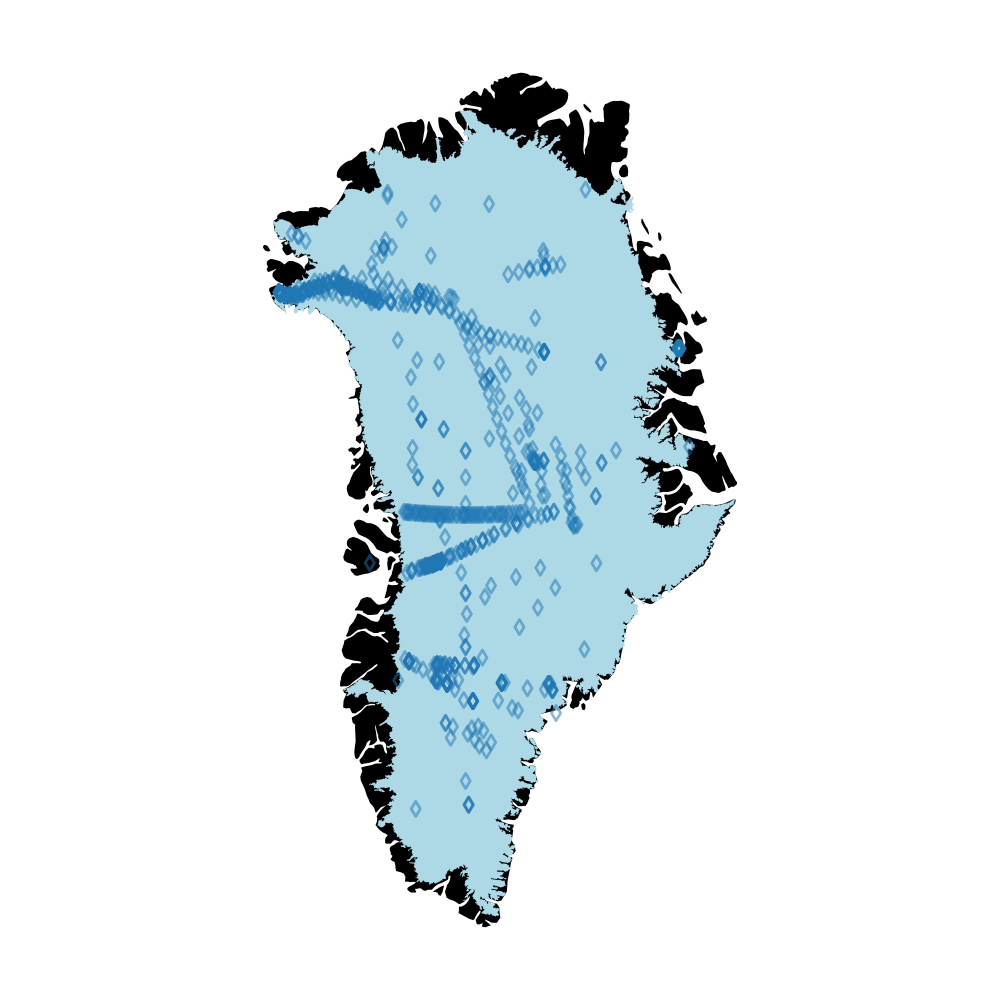
\includegraphics[width=0.45\textwidth]{figures/density_map_greenland.png}
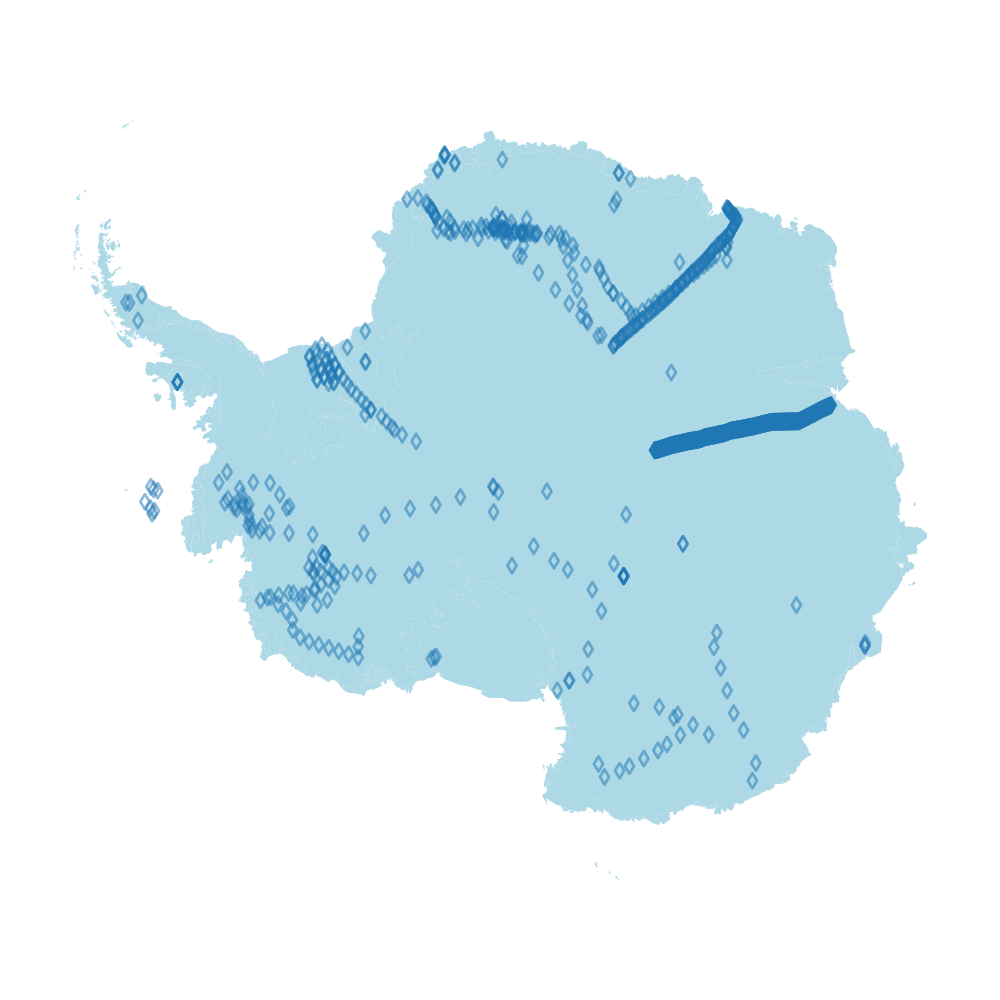
\includegraphics[width=0.45\textwidth]{figures/density_map_antarctica.png}
\end{figure}

\begin{figure}[!htb]
\caption{Composition of the density dataset in Greenland}
\centering
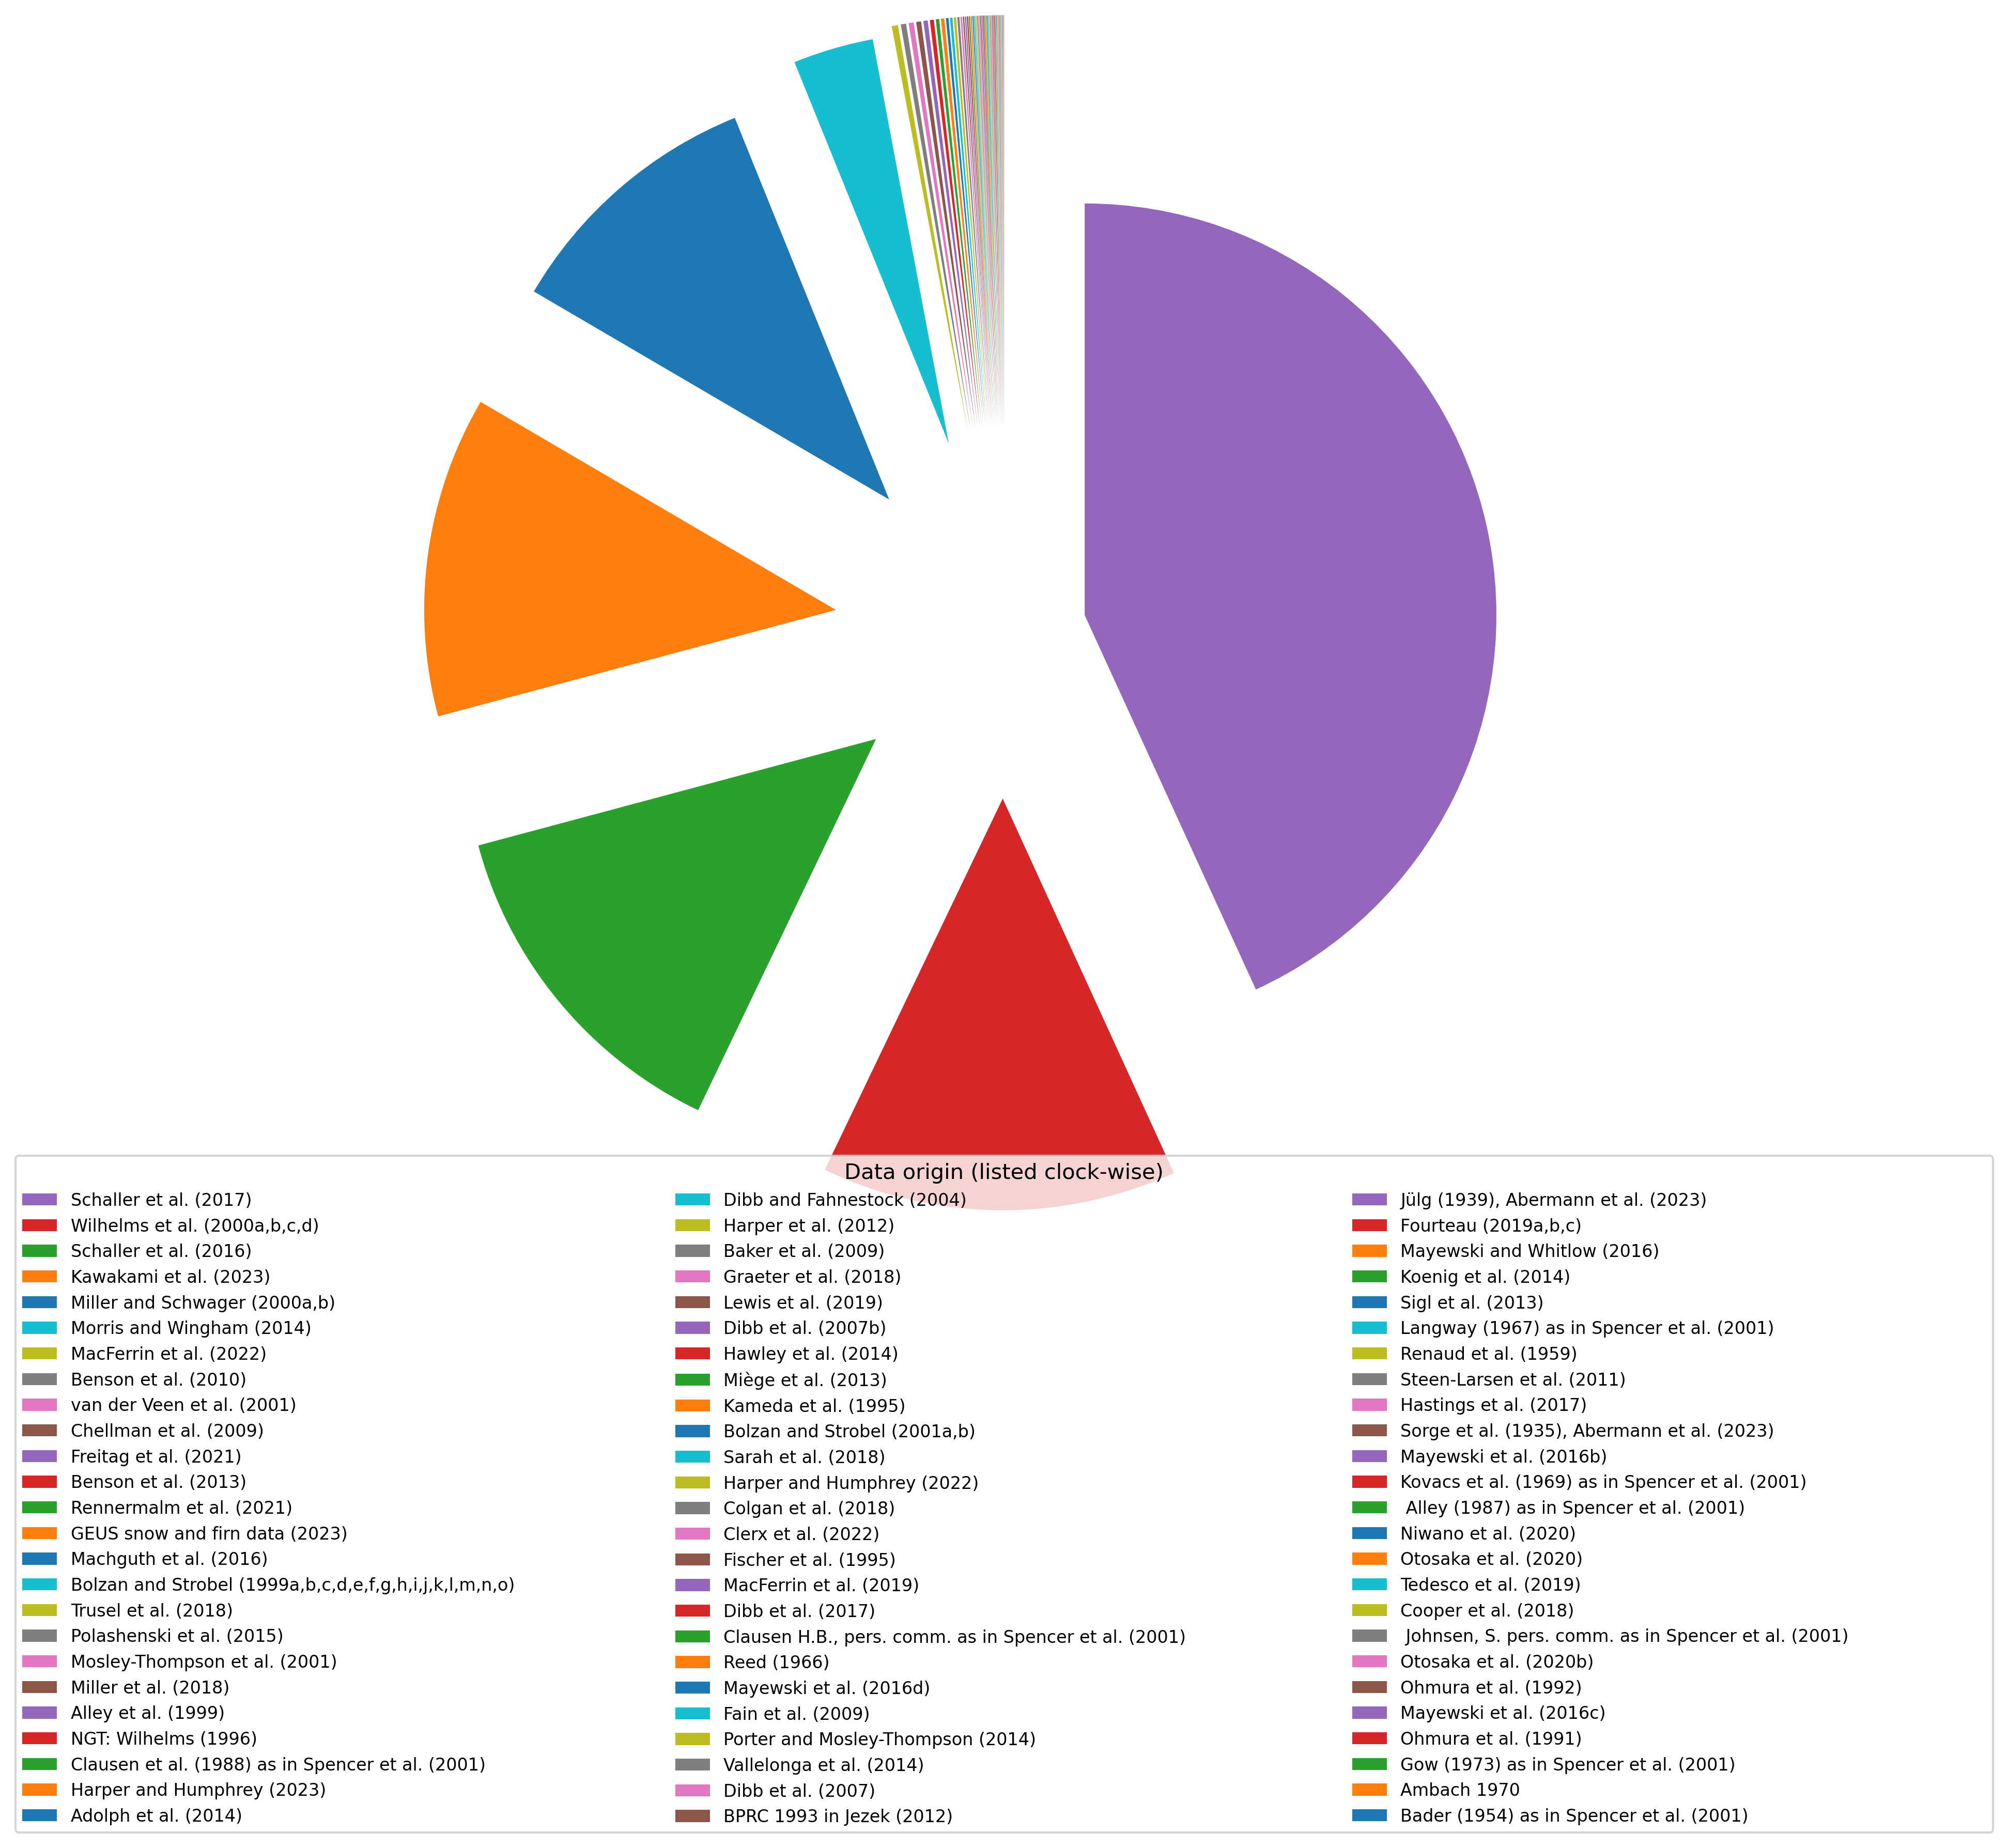
\includegraphics[width=0.8\textwidth]{figures/density_dataset_composition_greenland.png}
\end{figure}


\begin{figure}[!htb]
\caption{Composition of the density dataset in Antarctica}
\centering
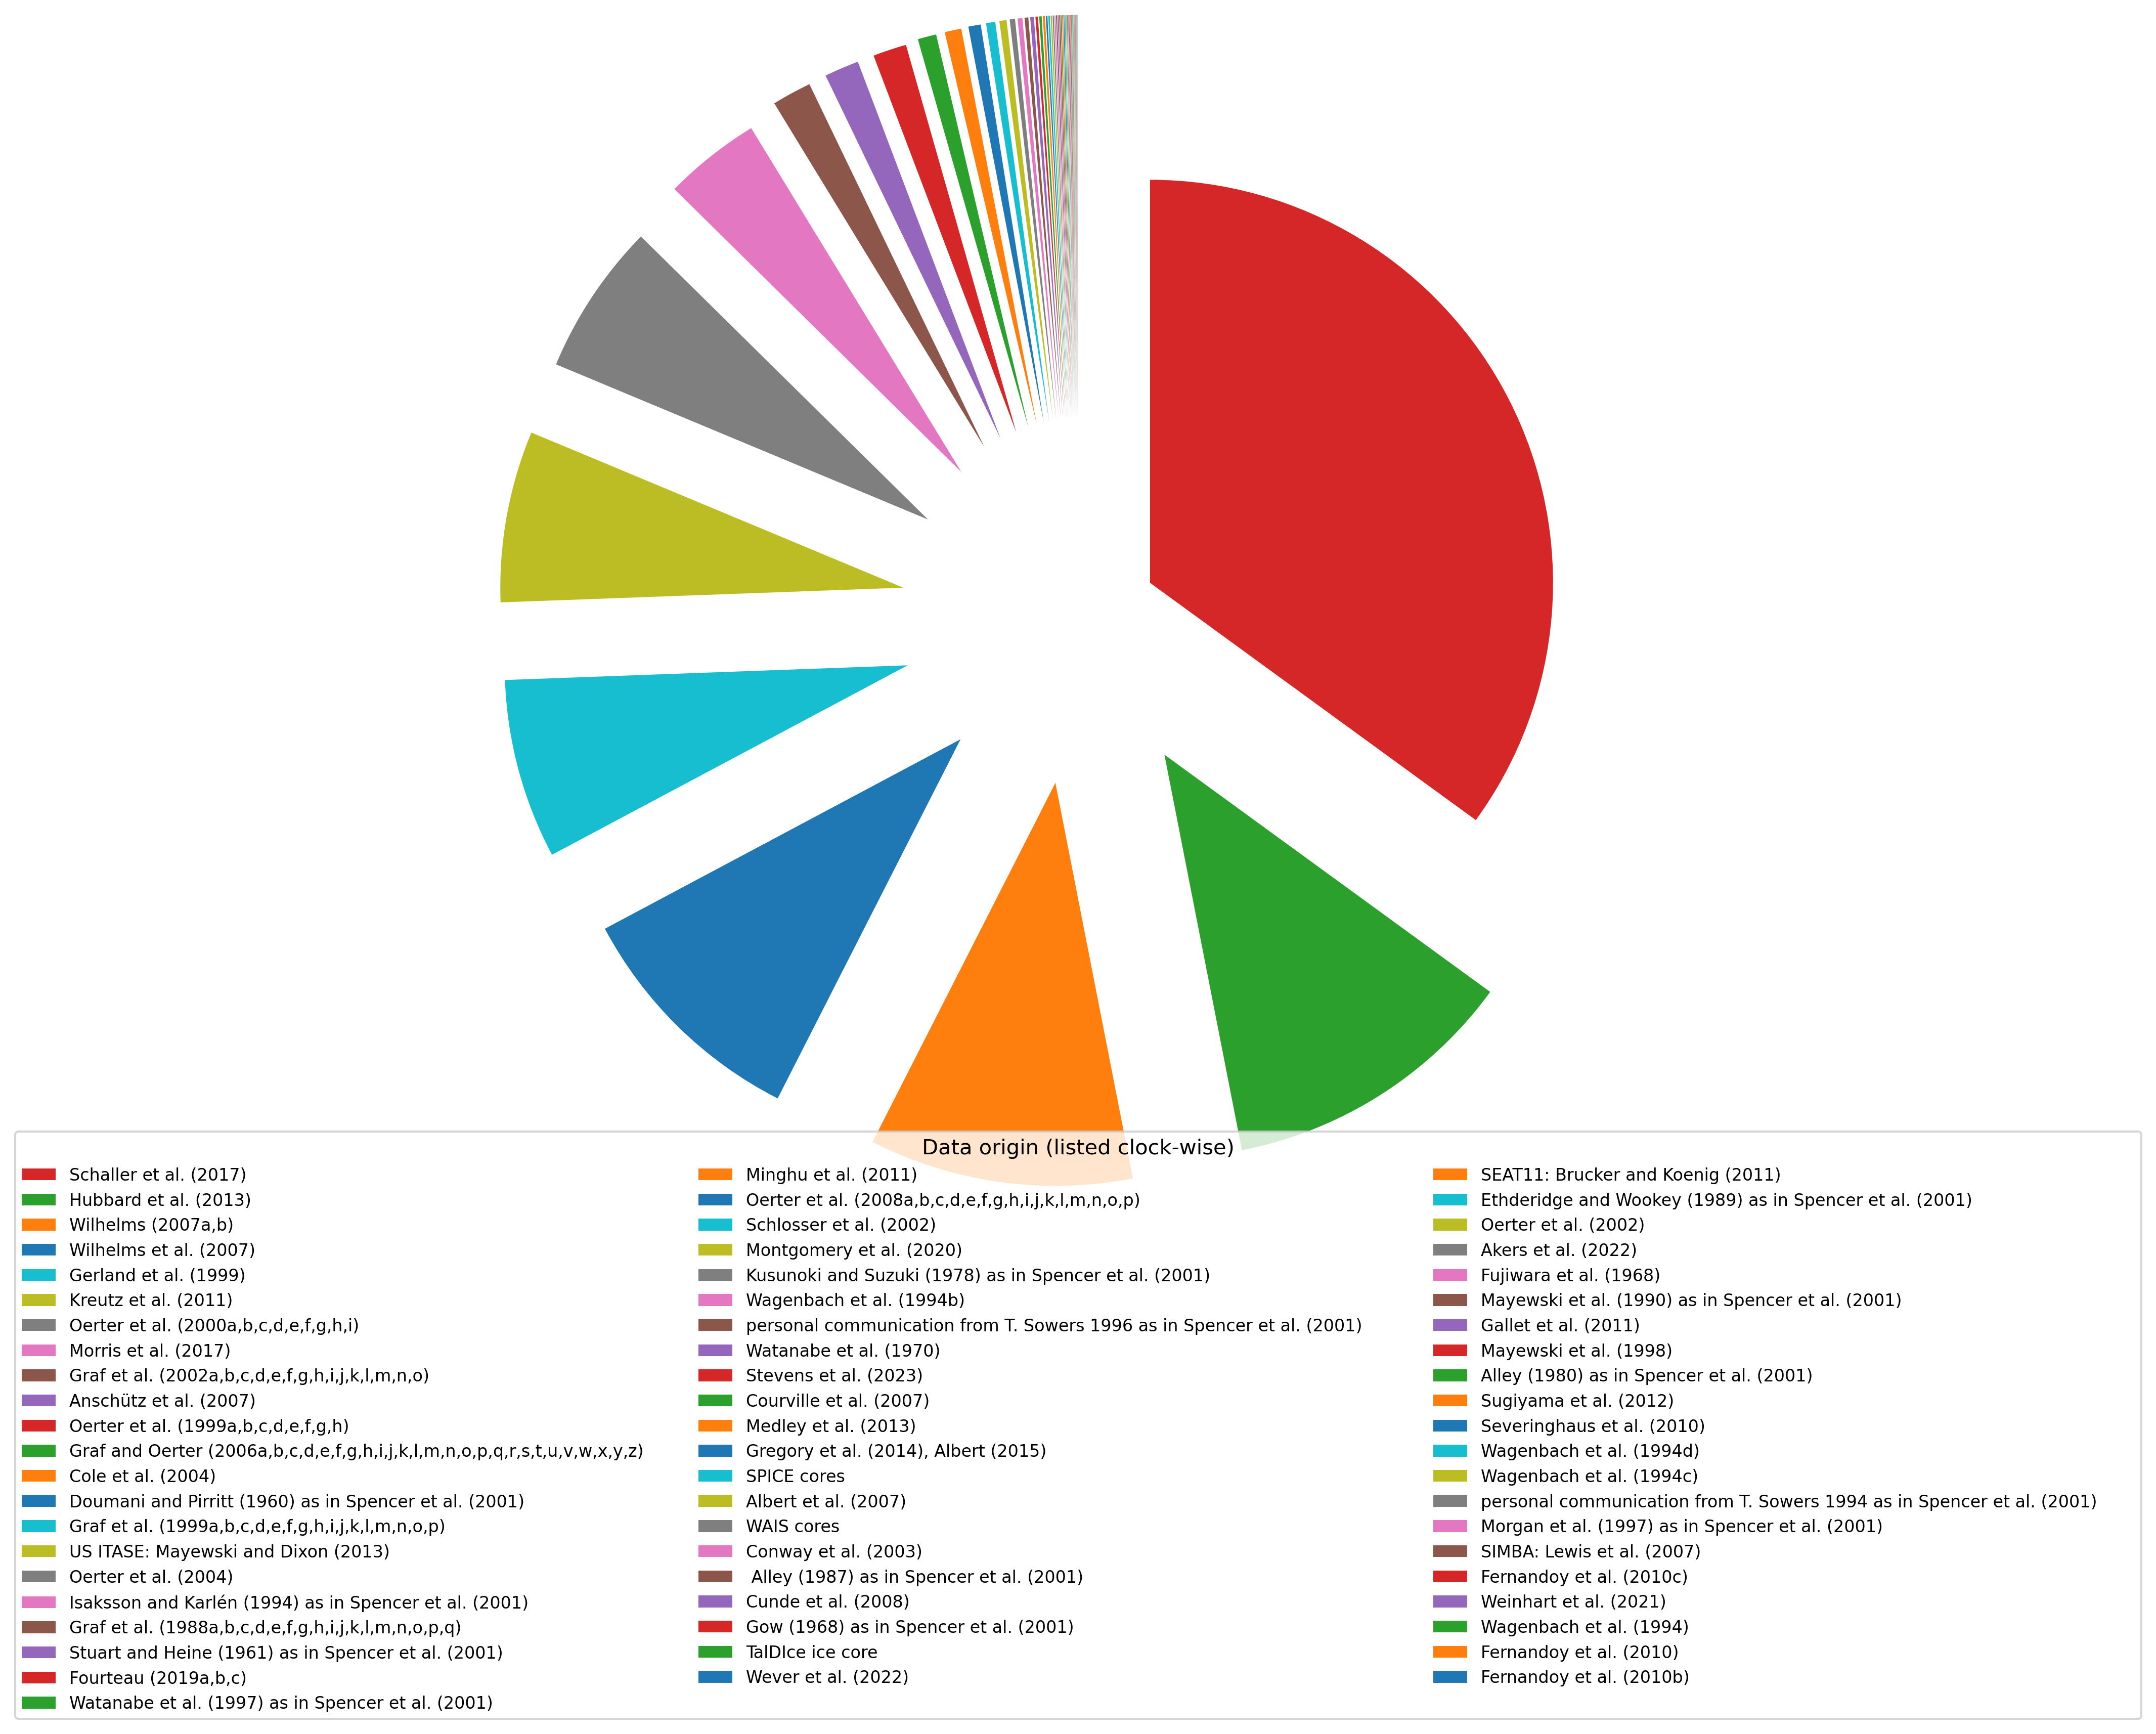
\includegraphics[width=0.8\textwidth]{figures/density_dataset_composition_antarctica.png}
\end{figure}

\FloatBarrier
\subsection{SMB}
\small
\csvautolongtable[
 table head=\caption{Origins and temporal coverage of the SMB data in Greenland}\label{tab:comp_smb_gr}\\\hline
               \csvlinetotablerow\\\hline
               \endfirsthead\hline
               \csvlinetotablerow\\\hline
               \endhead\hline
               \endfoot,
               respect all]{tables/composition_SMB_greenland.csv}
\small
\csvautolongtable[
 table head=\caption{Origins and temporal coverage of the SMB data in Antarctica}\label{tab:comp_smb_ant}\\\hline
               \csvlinetotablerow\\\hline
               \endfirsthead\hline
               \csvlinetotablerow\\\hline
               \endhead\hline
               \endfoot,
               respect all]{tables/composition_SMB_antarctica.csv}

\begin{figure}[!htb]
\caption{Spatial distribution of the SMB measurements}
\centering
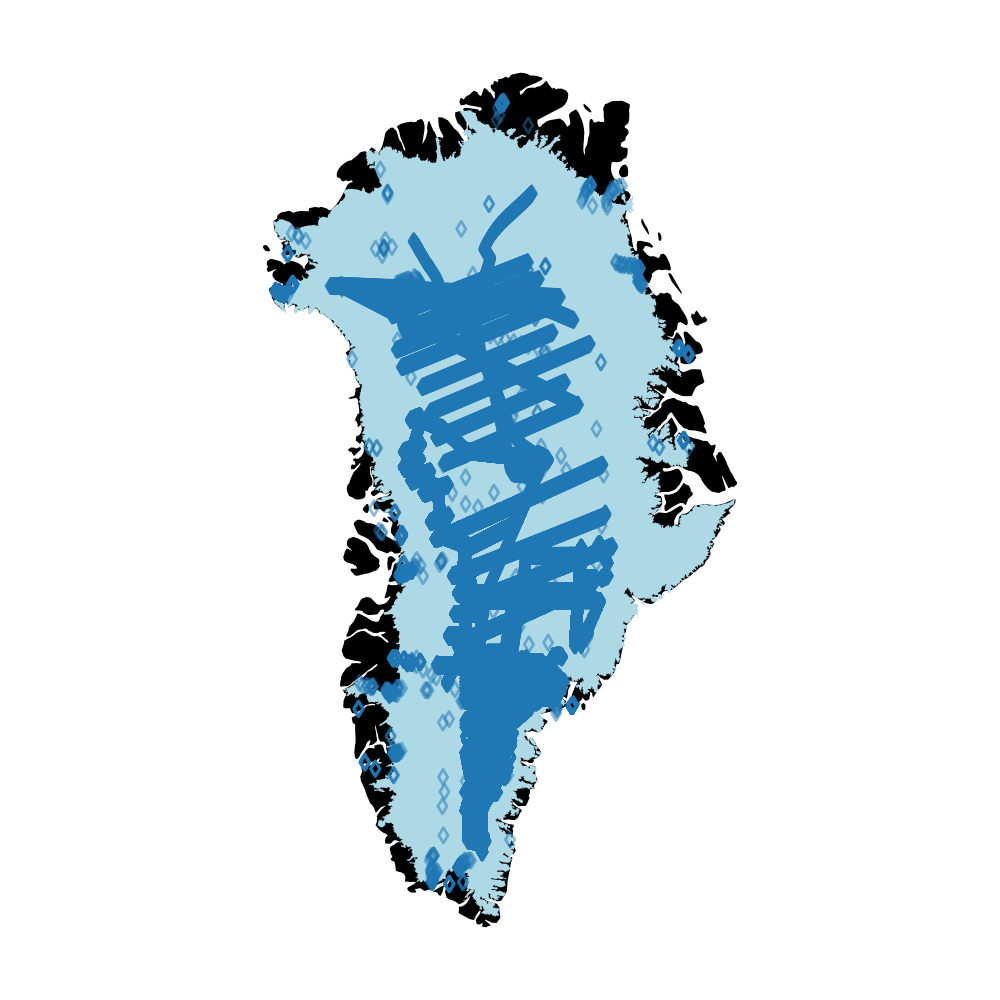
\includegraphics[width=0.45\textwidth]{figures/SMB_map_greenland.png}
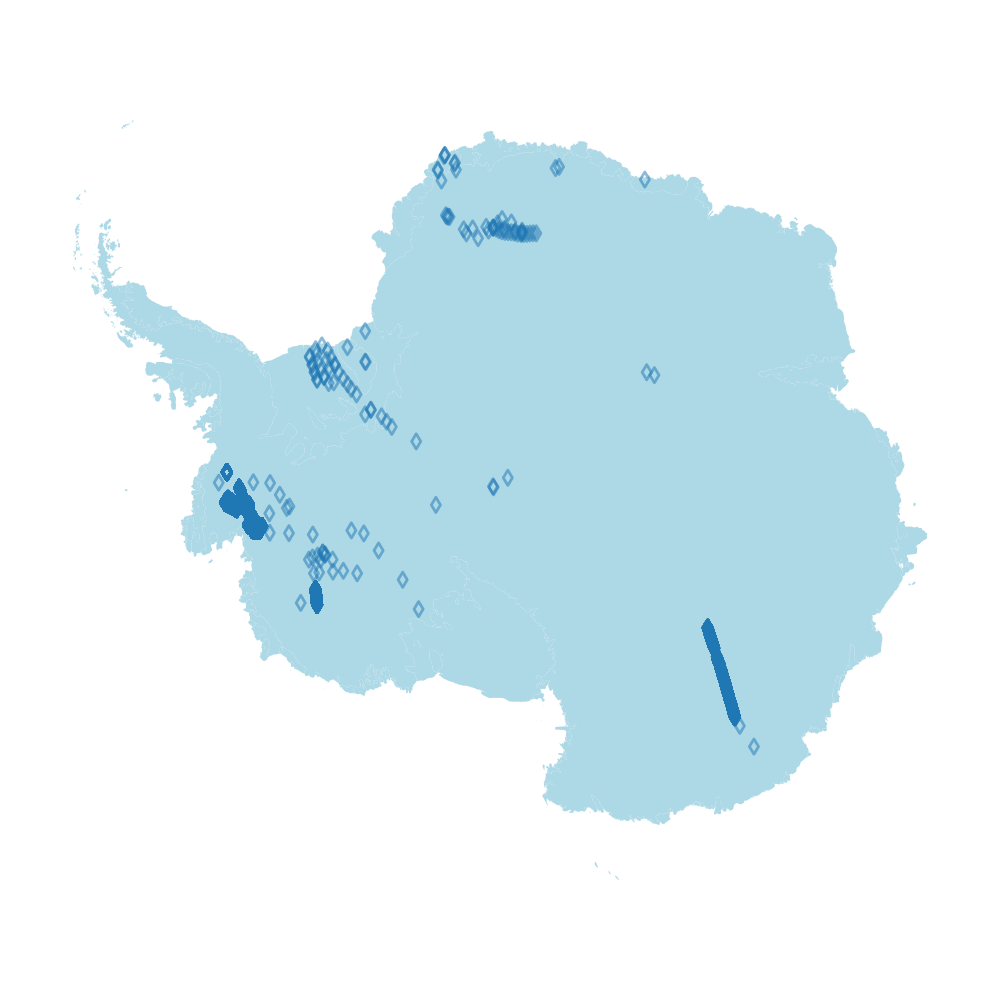
\includegraphics[width=0.45\textwidth]{figures/SMB_map_antarctica.png}
\end{figure}

\begin{figure}[!htb]
\caption{Composition of the SMB dataset in Greenland}
\centering
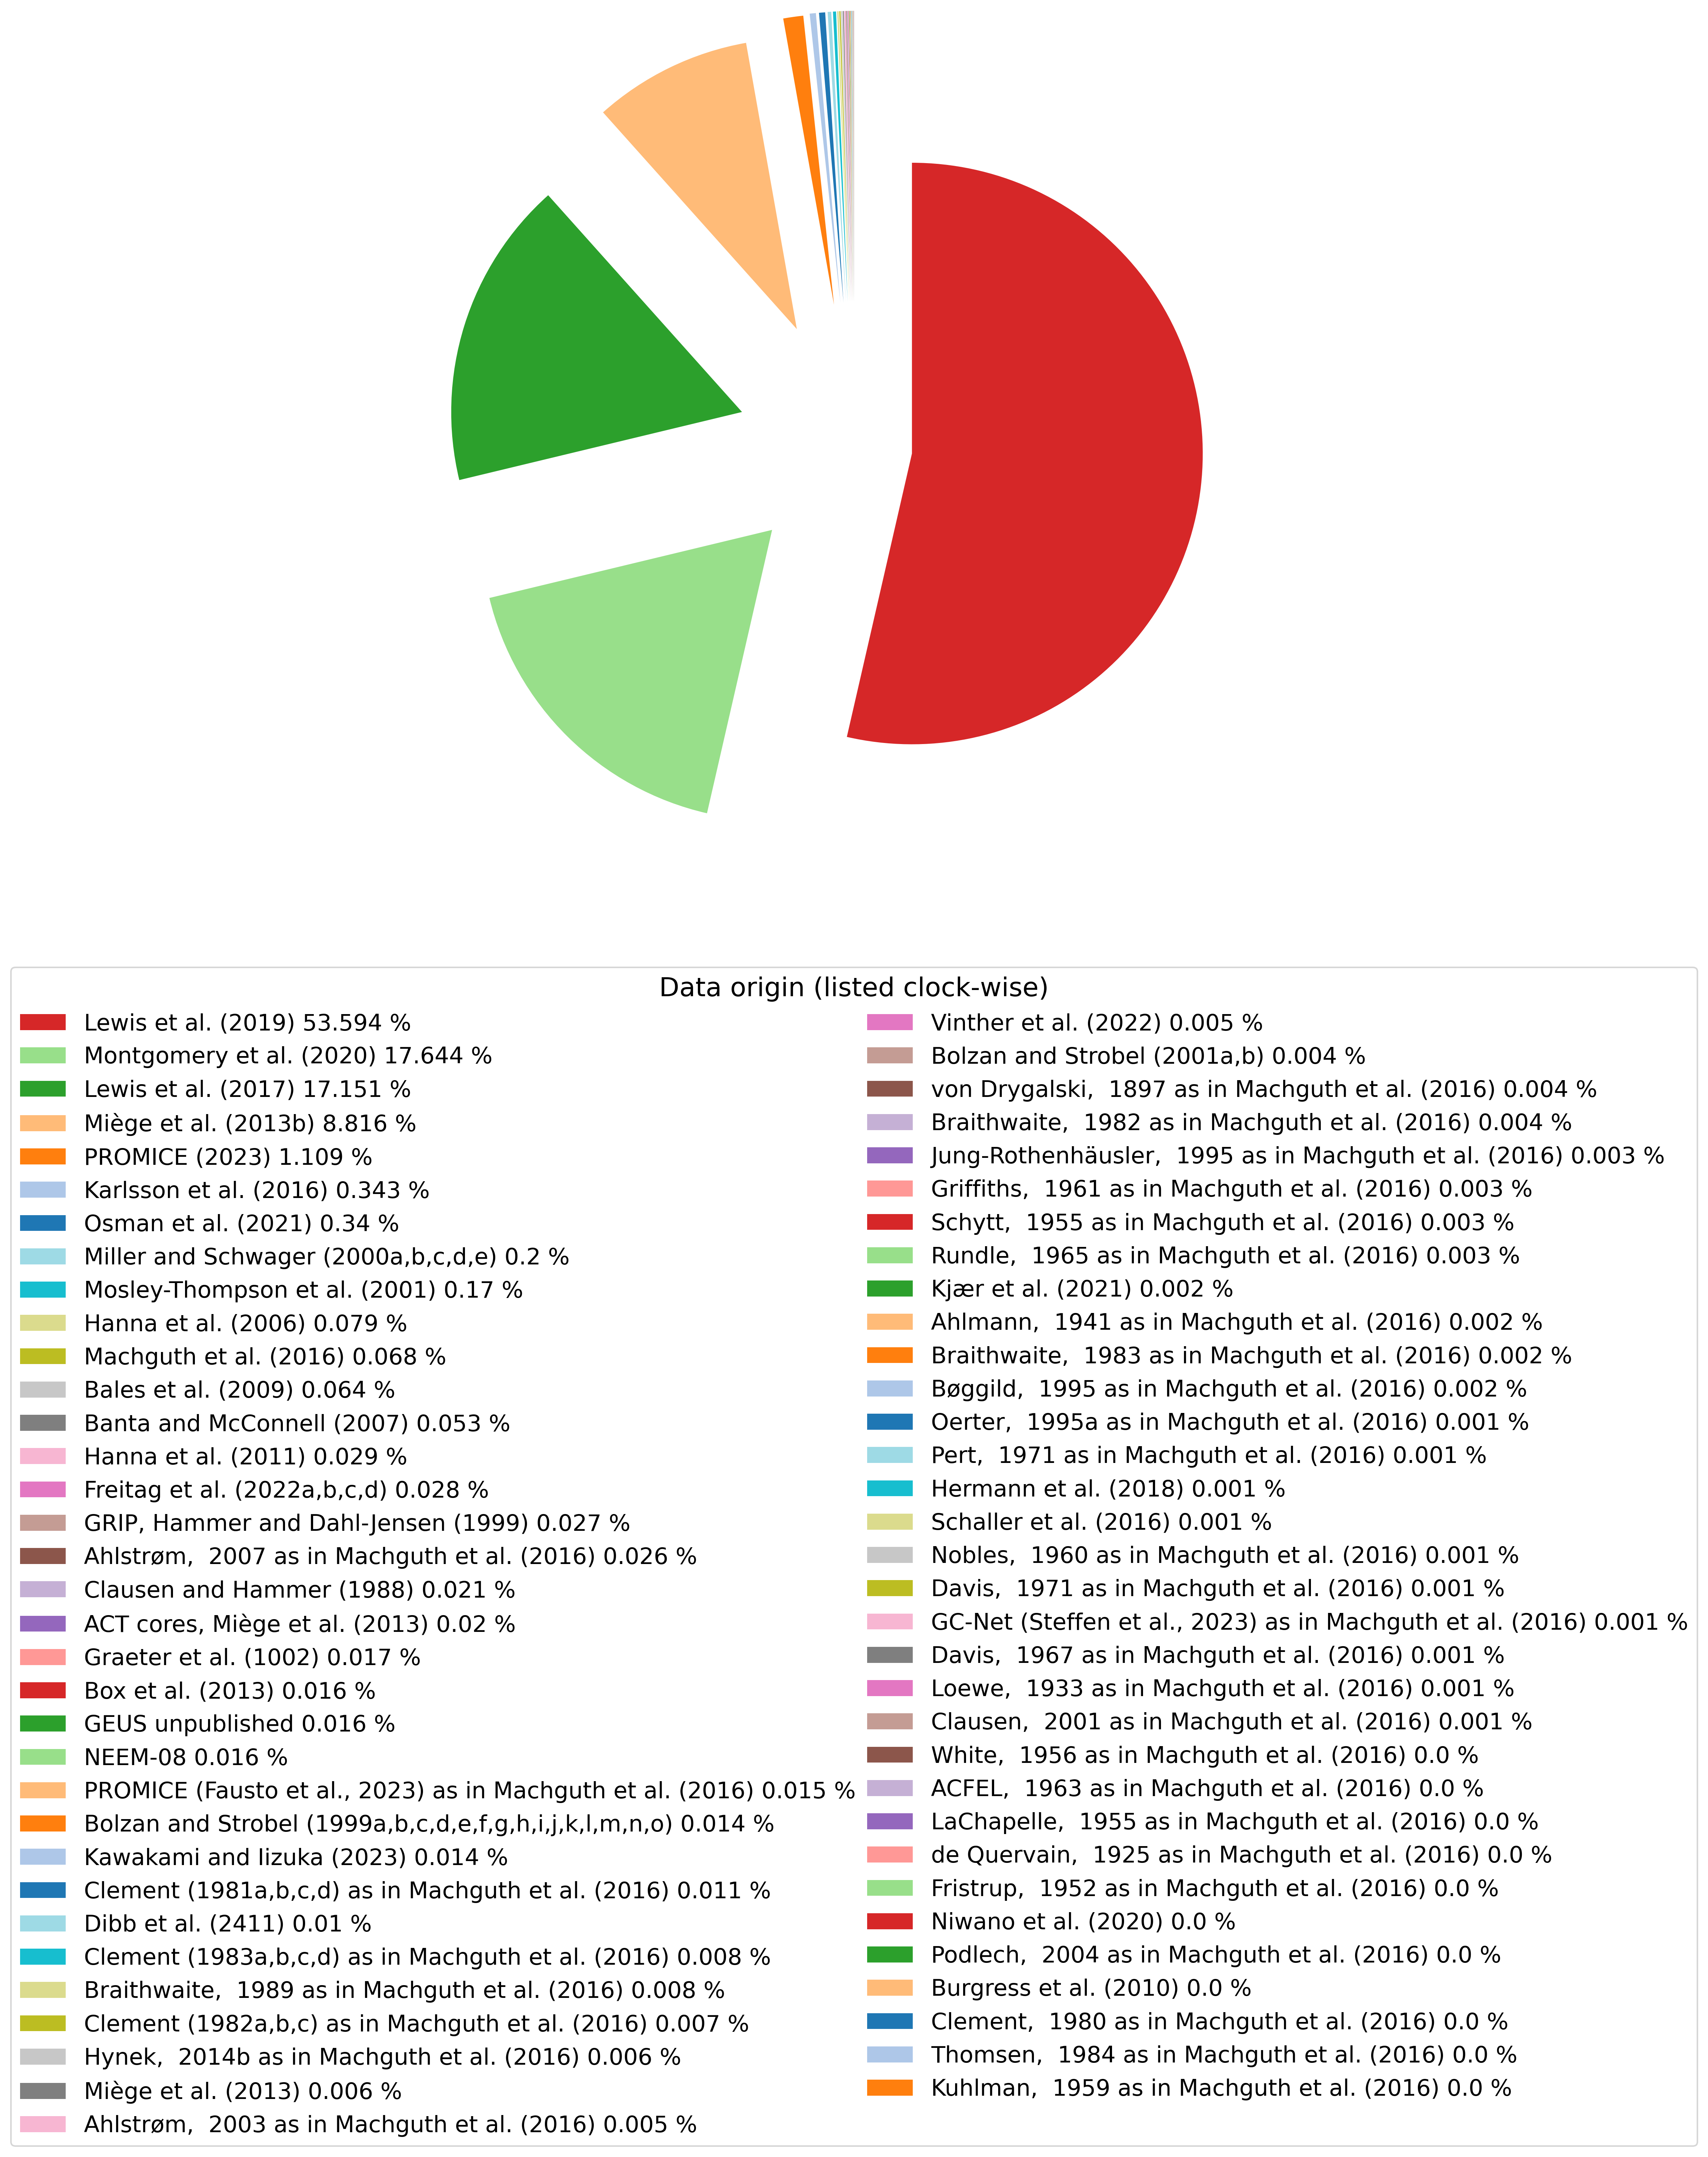
\includegraphics[width=0.8\textwidth]{figures/SMB_dataset_composition_greenland.png}
\end{figure}


\begin{figure}[!htb]
\caption{Composition of the SMB dataset in Antarctica}
\centering
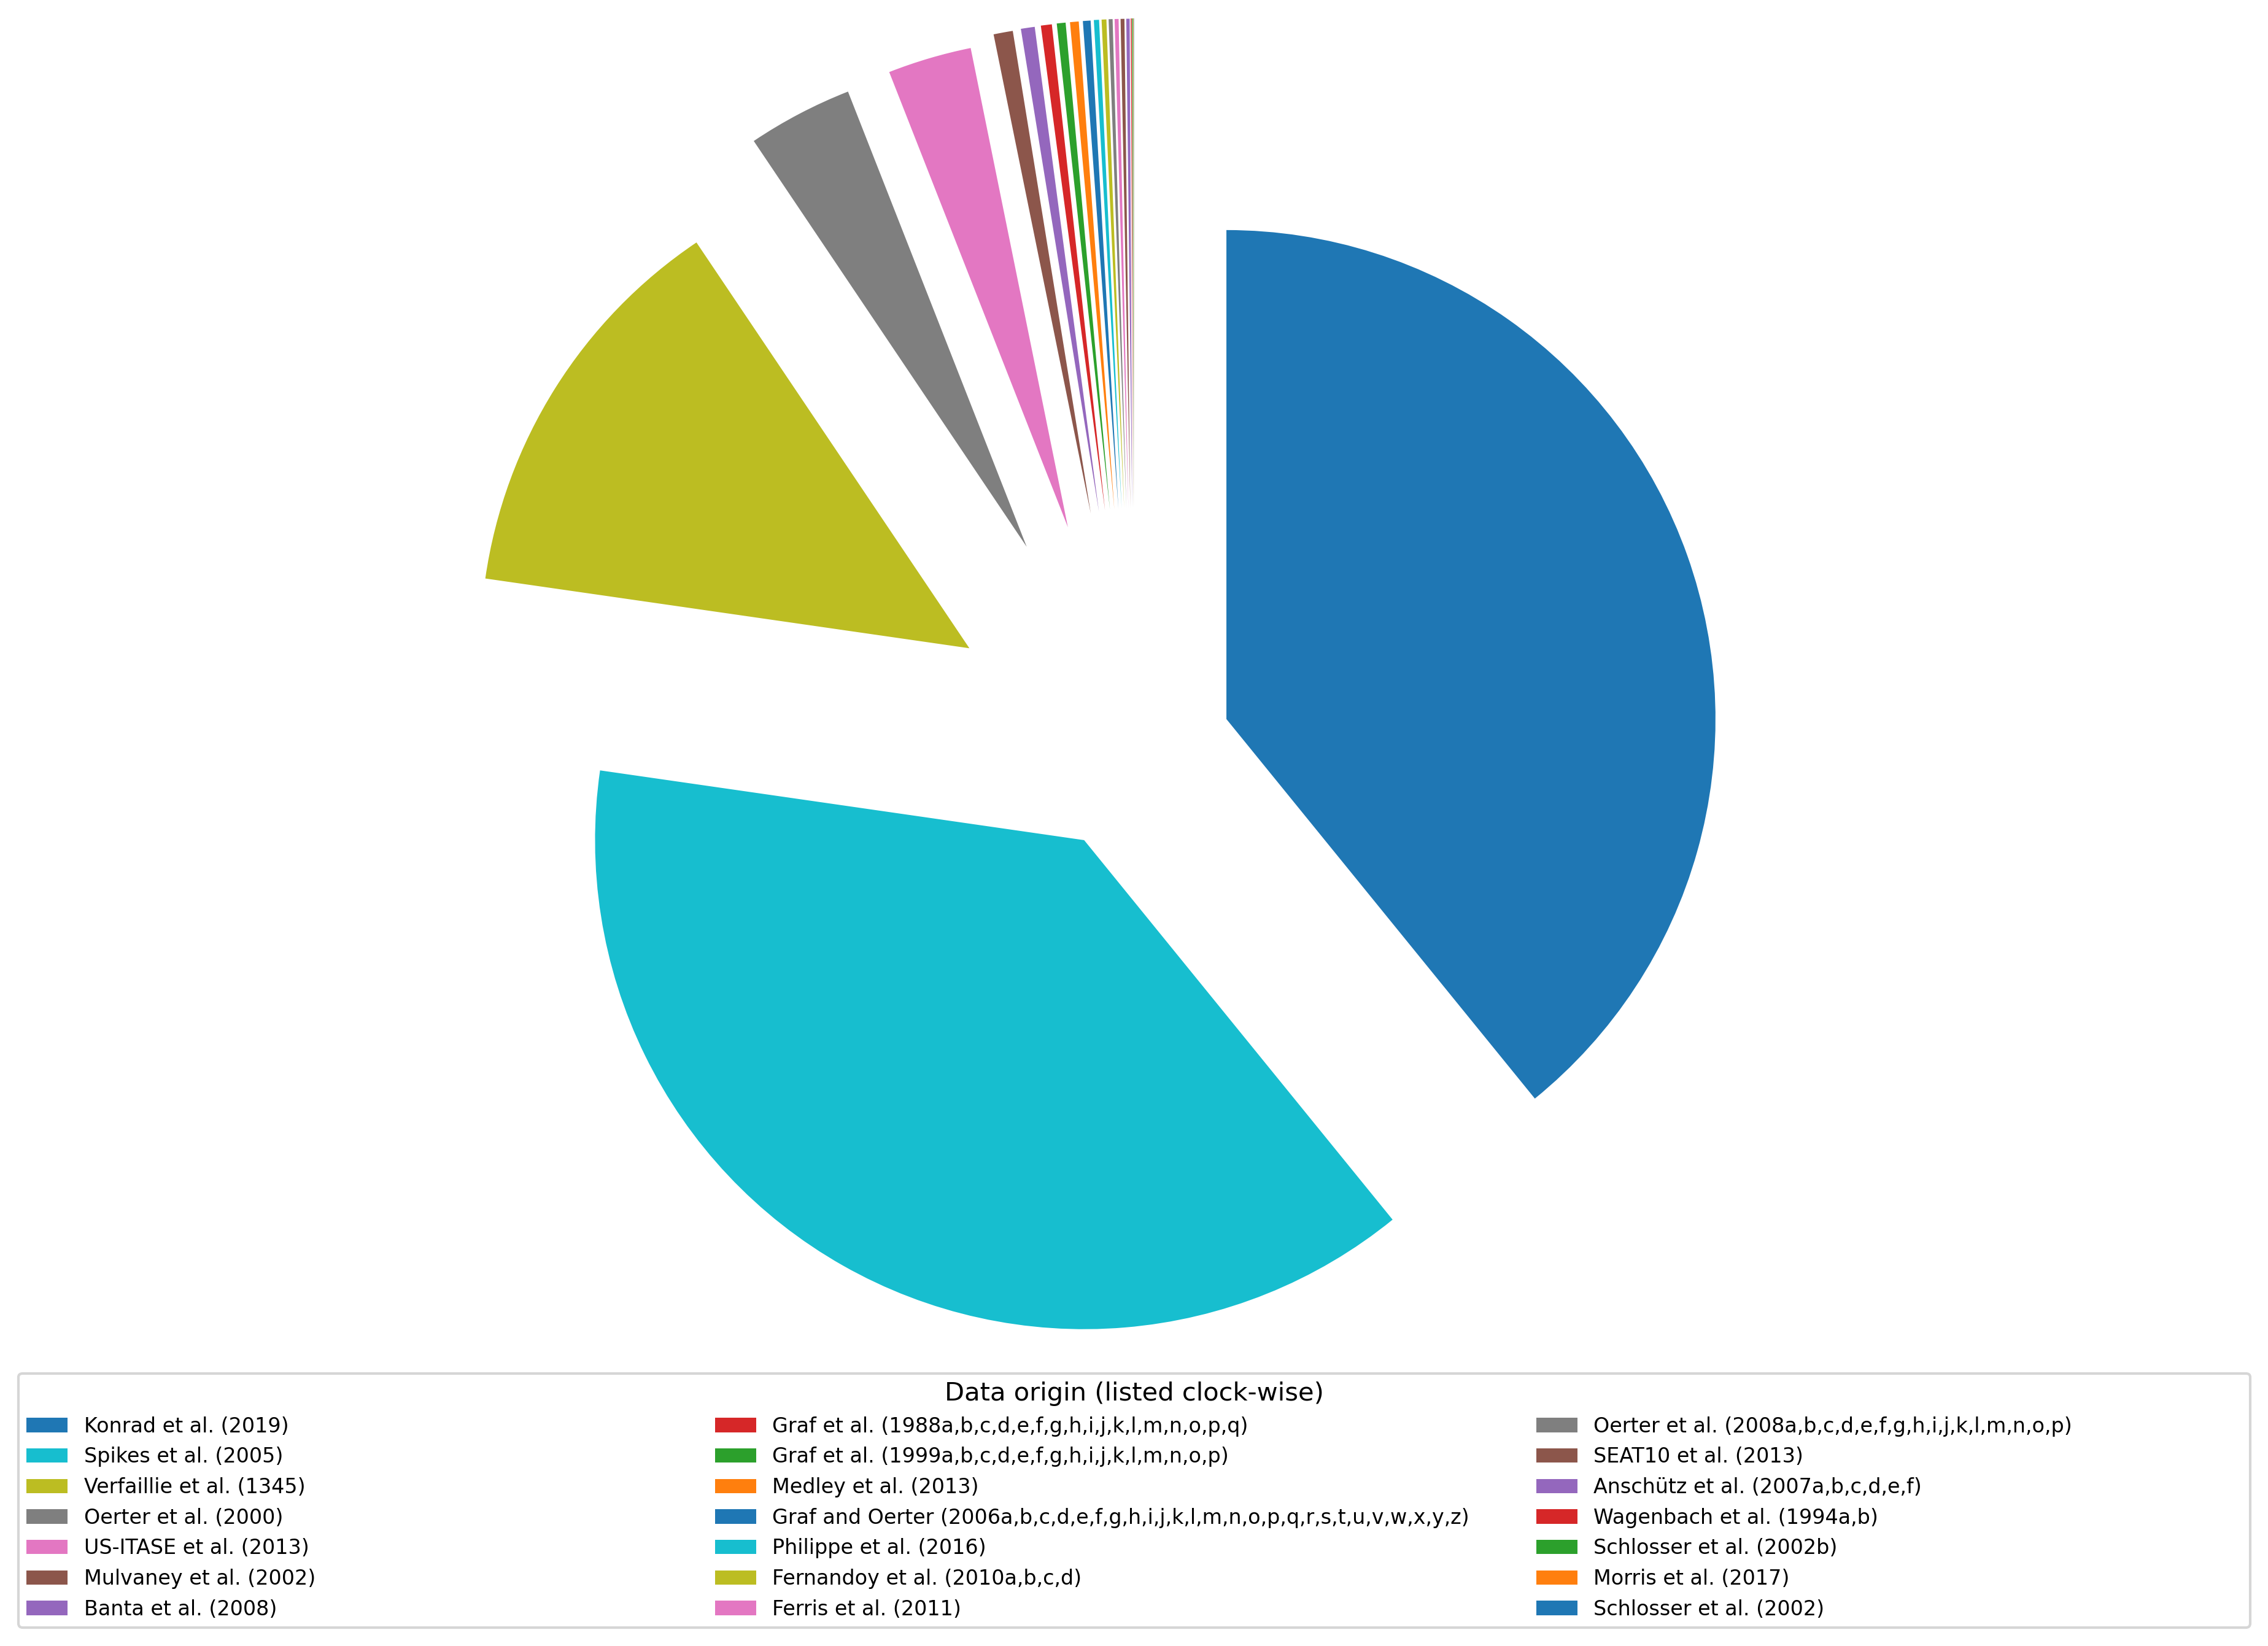
\includegraphics[width=0.8\textwidth]{figures/SMB_dataset_composition_antarctica.png}
\end{figure}

\FloatBarrier
\subsection{Temperature}
\small
\csvautolongtable[
 table head=\caption{Origins and temporal coverage of the temperature data in Greenland}\label{tab:comp_temp_gr}\\\hline
               \csvlinetotablerow\\\hline
               \endfirsthead\hline
               \csvlinetotablerow\\\hline
               \endhead\hline
               \endfoot,
               respect all]{tables/composition_temperature_greenland.csv}
\small
\csvautolongtable[
 table head=\caption{Origins and temporal coverage of the temperature data in Antarctica}\label{tab:comp_temp_ant}\\\hline
               \csvlinetotablerow\\\hline
               \endfirsthead\hline
               \csvlinetotablerow\\\hline
               \endhead\hline
               \endfoot,
               respect all]{tables/composition_temperature_antarctica.csv}

\begin{figure}[!htb]
\caption{Spatial distribution of the temperature measurements}
\centering
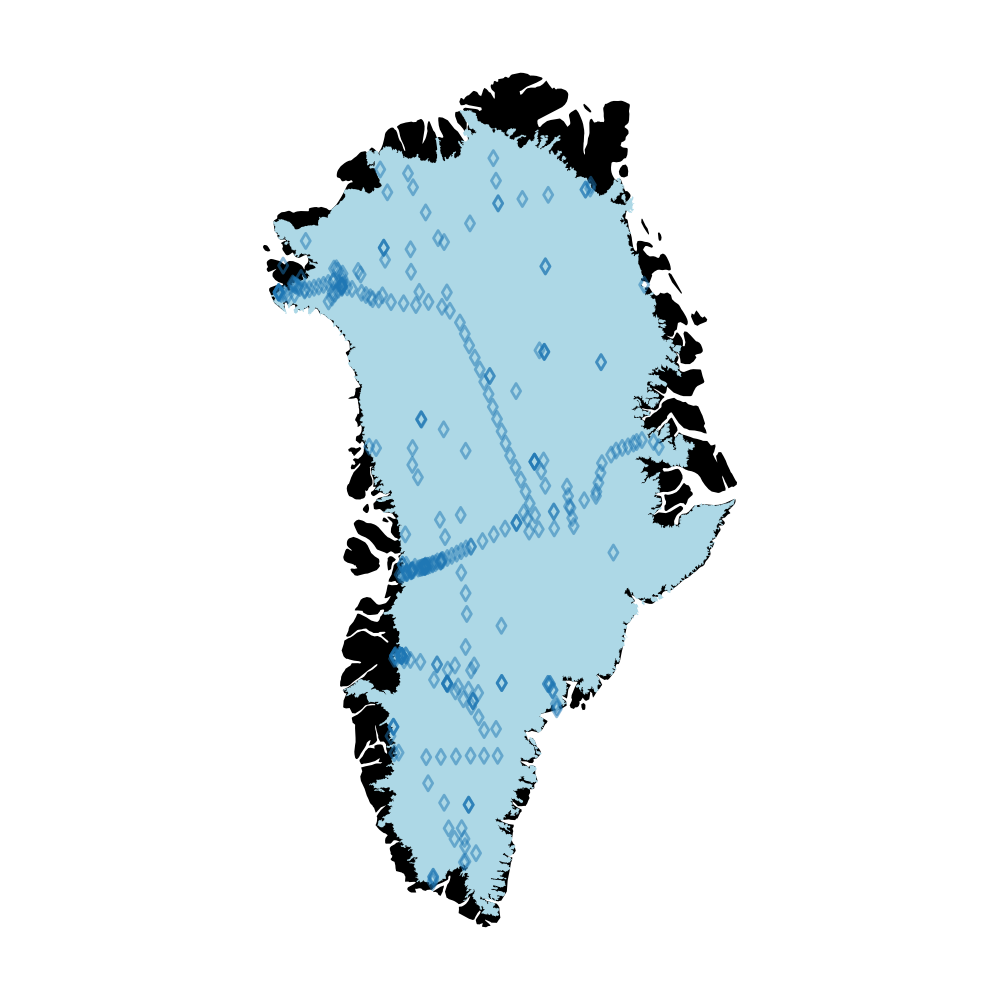
\includegraphics[width=0.45\textwidth]{figures/temperature_map_greenland.png}
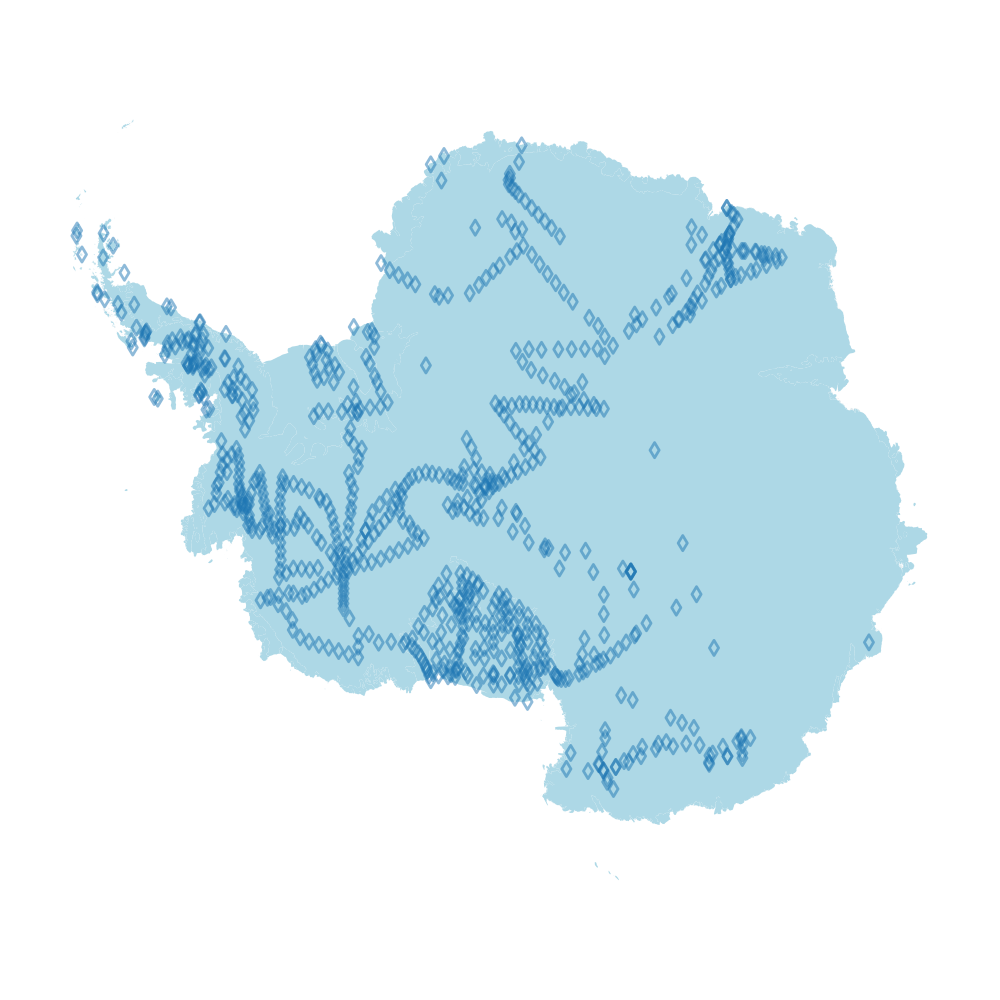
\includegraphics[width=0.45\textwidth]{figures/temperature_map_antarctica.png}
\end{figure}

\begin{figure}[!htb]
\caption{Composition of the temperature dataset in Greenland}
\centering
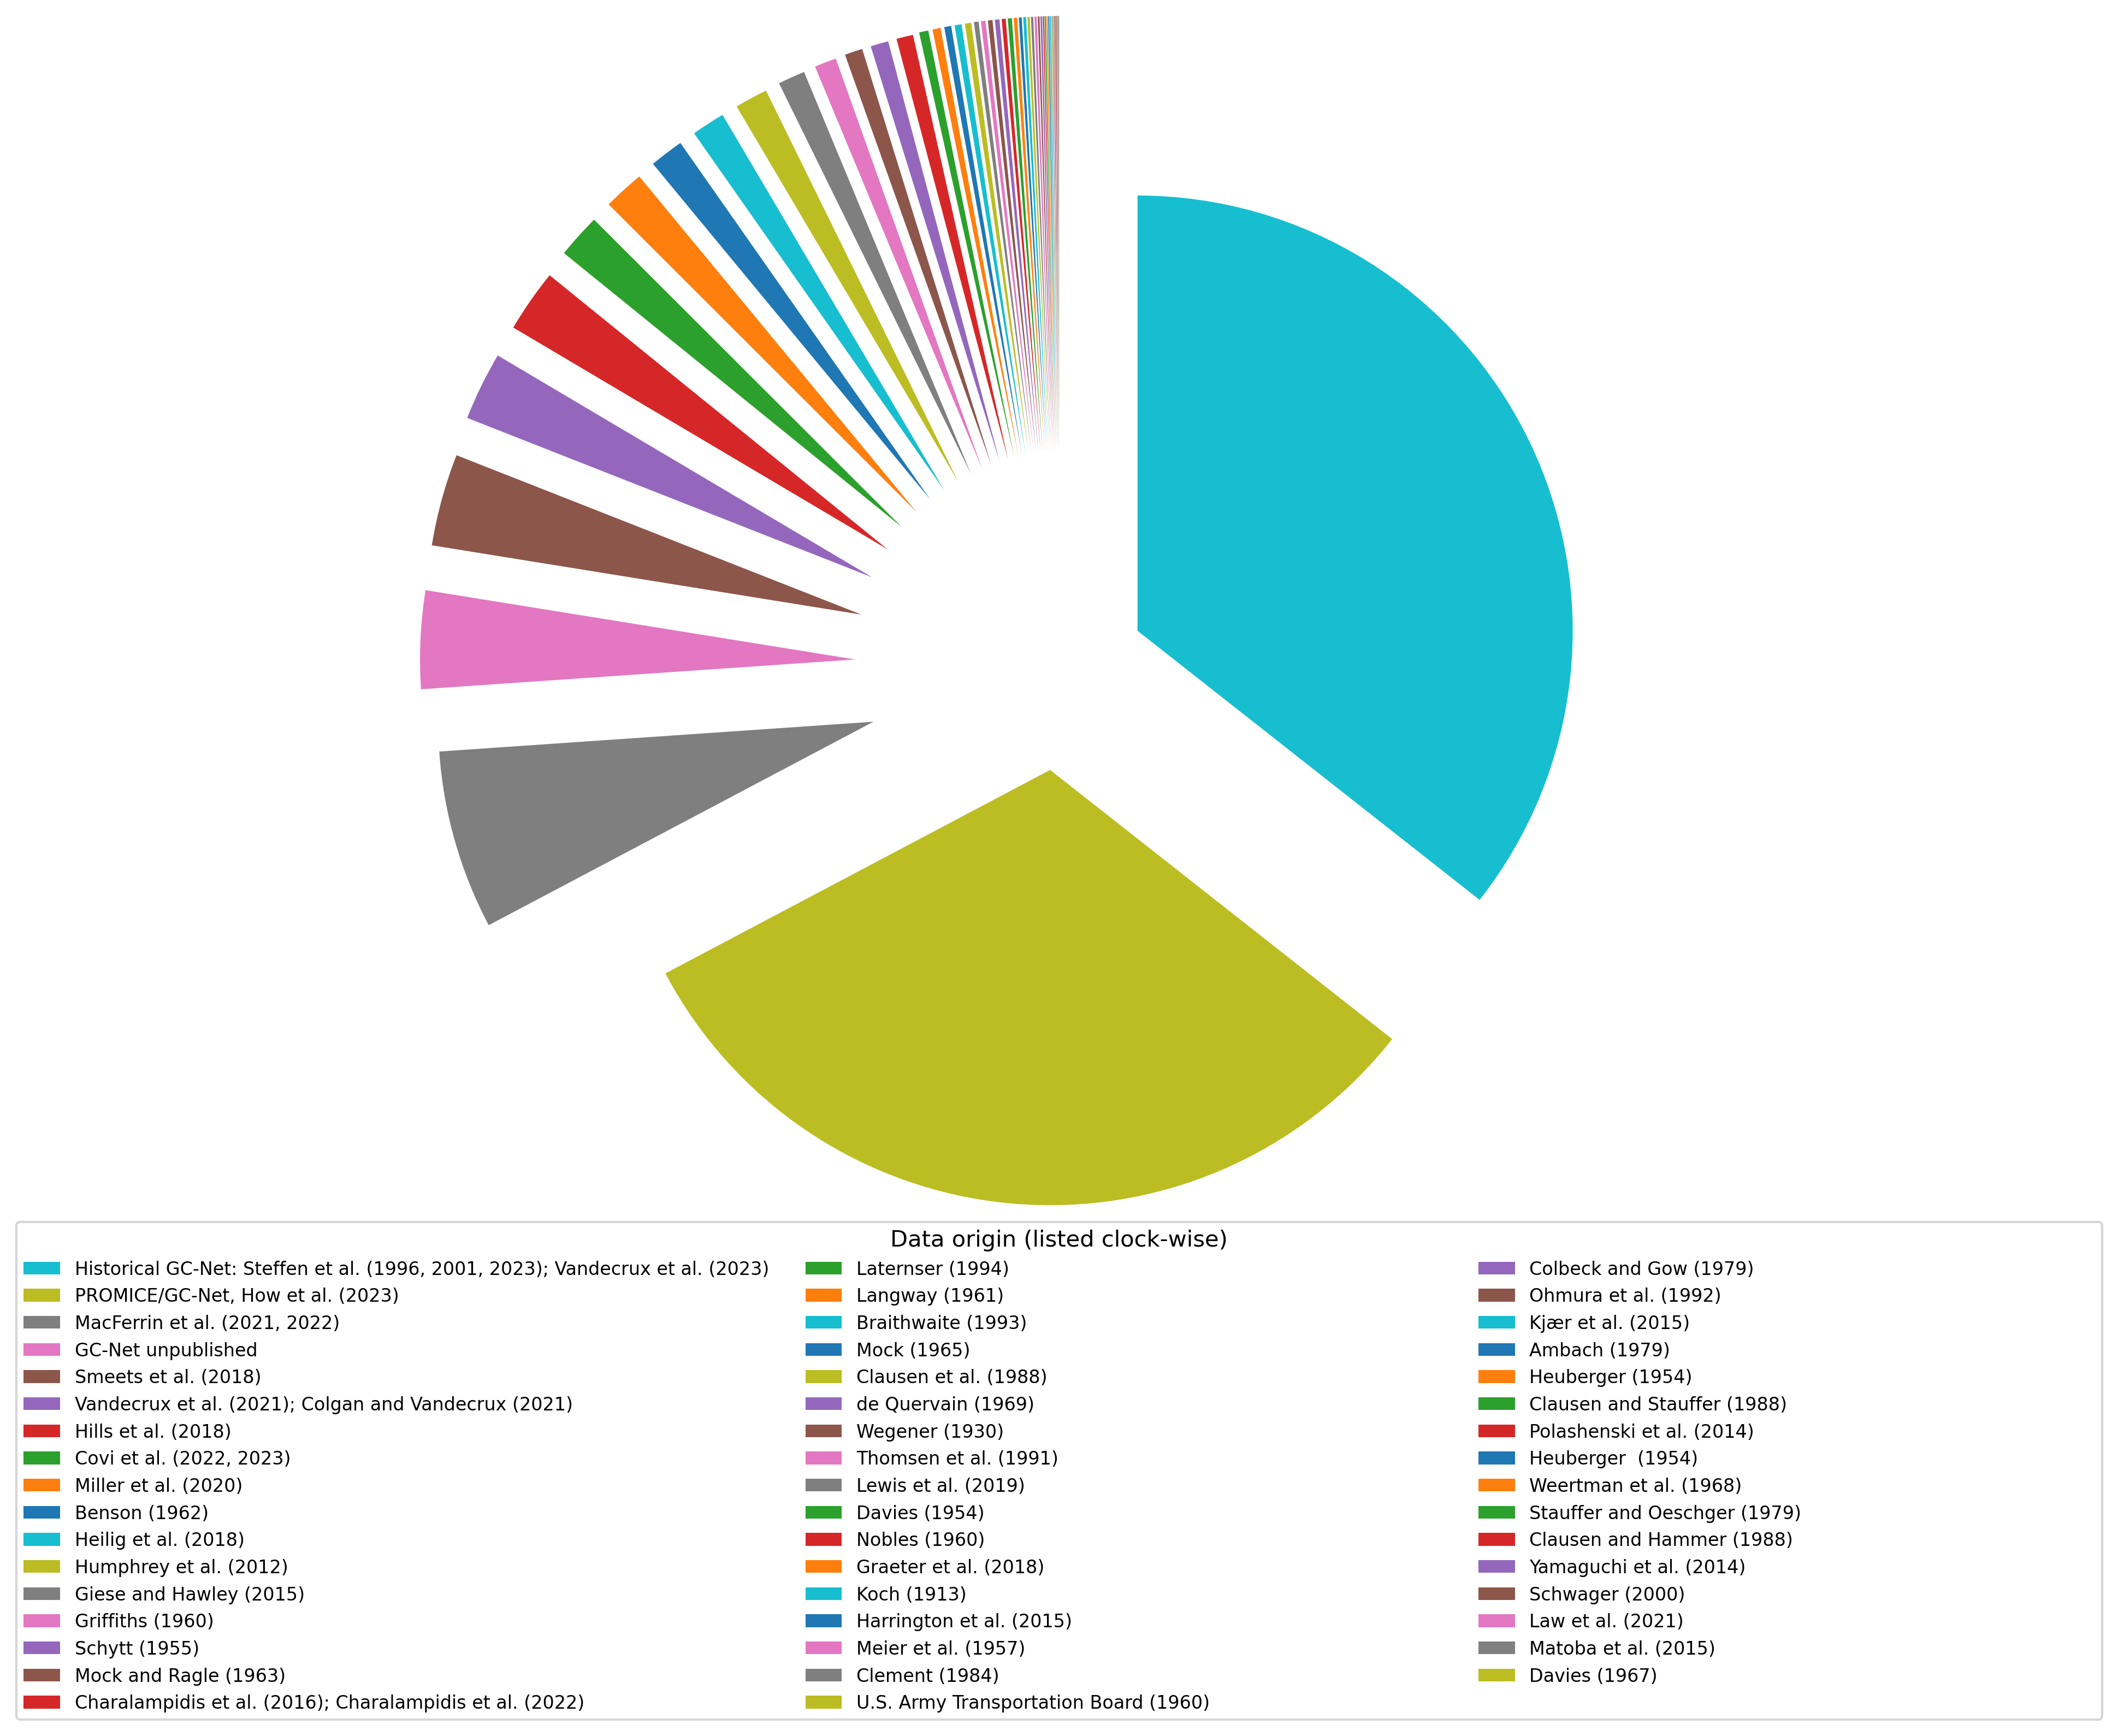
\includegraphics[width=0.8\textwidth]{figures/temperature_dataset_composition_greenland.png}
\end{figure}


\begin{figure}[!htb]
\caption{Composition of the temperature dataset in Antarctica}
\centering
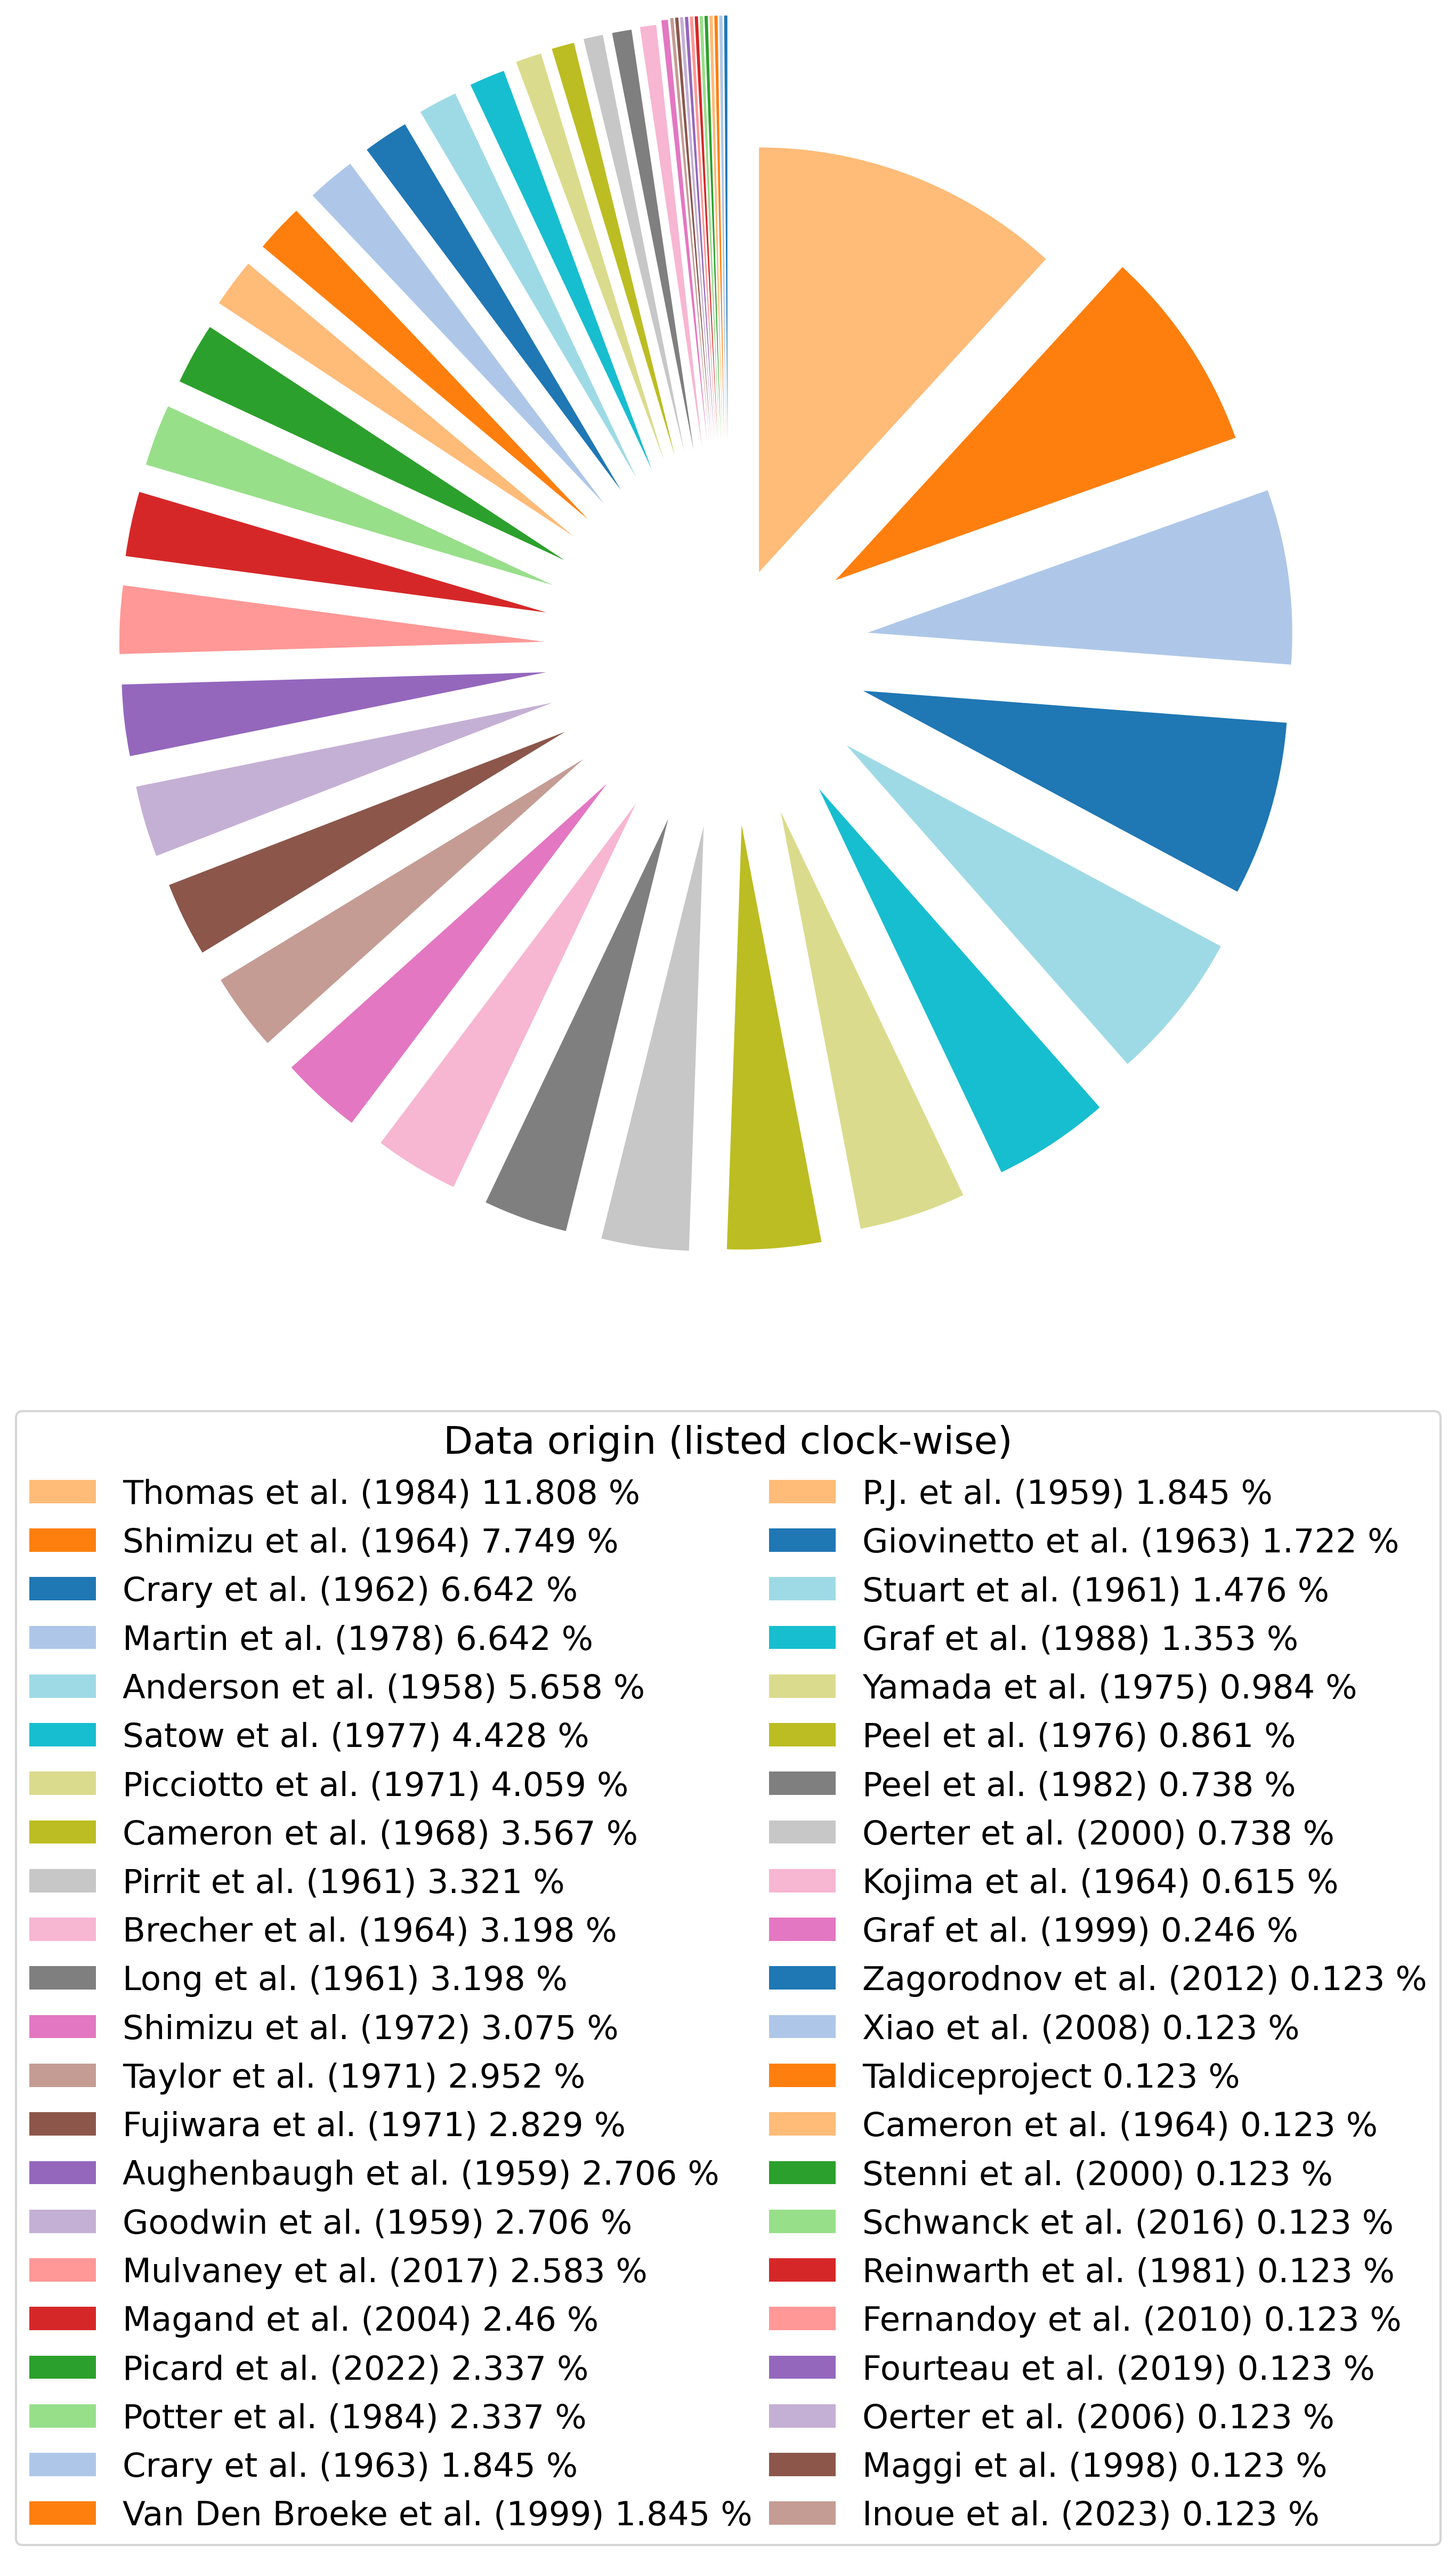
\includegraphics[width=0.8\textwidth]{figures/temperature_dataset_composition_antarctica.png}
\end{figure}

%\conclusions  %% \conclusions[modified heading if necessary]
%\dataavailability{TEXT} %% use this section when having only data sets available
%\codedataavailability{TEXT} 
%\noappendix       %% use this to mark the end of the appendix section
%\authorcontribution{TEXT} 
%\begin{acknowledgements}
%TEXT
%\end{acknowledgements}
%% REFERENCES
%% The reference list is compiled as follows:
%\begin{thebibliography}{}
%\bibitem[AUTHOR(YEAR)]{LABEL1}
%REFERENCE 1
%\bibitem[AUTHOR(YEAR)]{LABEL2}
%REFERENCE 2
%\end{thebibliography}

\end{document}
